\documentclass[main.tex]{subfiles}
\begin{document}

\href{https://www2.seas.gwu.edu/~simhaweb/quantum/modules/module6/module6.html}{Module 6: Quantum circuits - gates}\\
\href{https://www2.seas.gwu.edu/~simhaweb/quantum/modules/module6/problems6.html}{Module 6: Quantum circuits - gates solved problems}

\subsection{Why circuits?}

    First, let's get a high-level view of what a quantum computation looks like shown in Figure \ref{fig:01circuit}.

    \begin{figure}
        \centering
        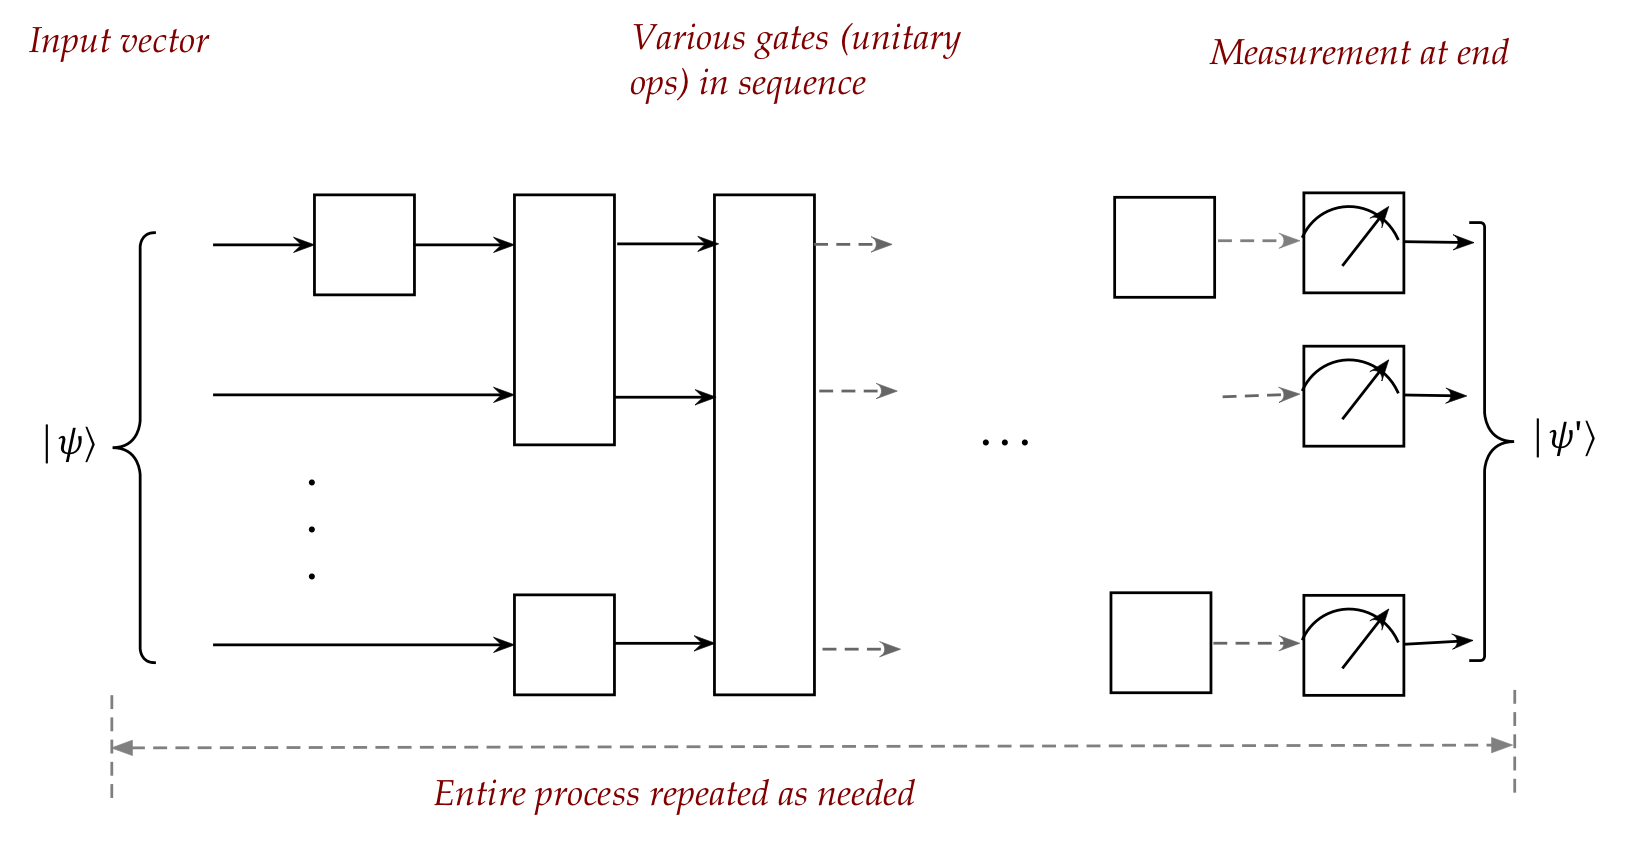
\includegraphics[width=5in]{notes/figs/n08/01circuit.png}
        \caption{Inputs Gate Measurement}
        \label{fig:01circuit}
    \end{figure}
    
    The input vector is often $|00 \ldots 0\rangle$. Quite frequently, the input vector is converted to
    
    $$
    |\psi\rangle=\frac{1}{\sqrt{2^{n}}}(|00 \ldots 0\rangle+|00 \ldots 1\rangle \ldots+|11 \ldots 1\rangle)
    $$
    
    the equal-superposition vector. This vector is then fed into a sequence of unitary operations (gates): The gates can be of various sizes. Each gate has the same number of outputs as inputs (It has to, else it won't be unitary.) A qubit that skips a gate is equivalently transformed by the $I$ (identity) gate. Measurement occurs at the end, resulting in a probabilistic outcome. The whole sequence is repeated often, and statistical analysis is performed on the collection of (probabilistic) outcomes. This is how a quantum algorithm works in the standard circuit model. Let's compare this with classical computing: First, compare with a simple calculator referenced in Figure \ref{fig:02calculator}.
    
    \begin{figure}
        \centering
        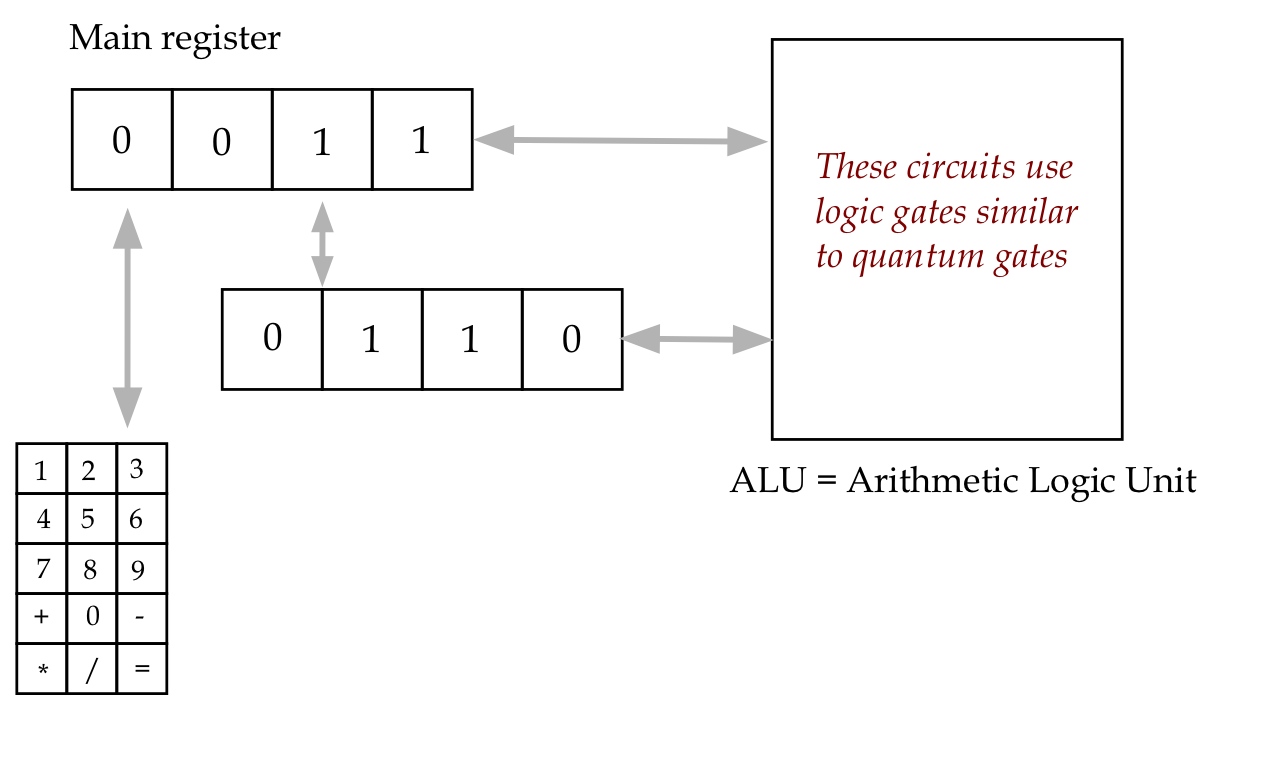
\includegraphics[width=4in]{notes/figs/n08/02calculator.png}
        \caption{simple calculator}
        \label{fig:02calculator}
    \end{figure}
    
    Here too, a set of binary values flows through a circuit. The circuit is itself a collection of (Boolean) gates. Now with something more capable (a 1950's computer) shown in Figure \ref{fig:03program}.
    
    \begin{figure}
        \centering
        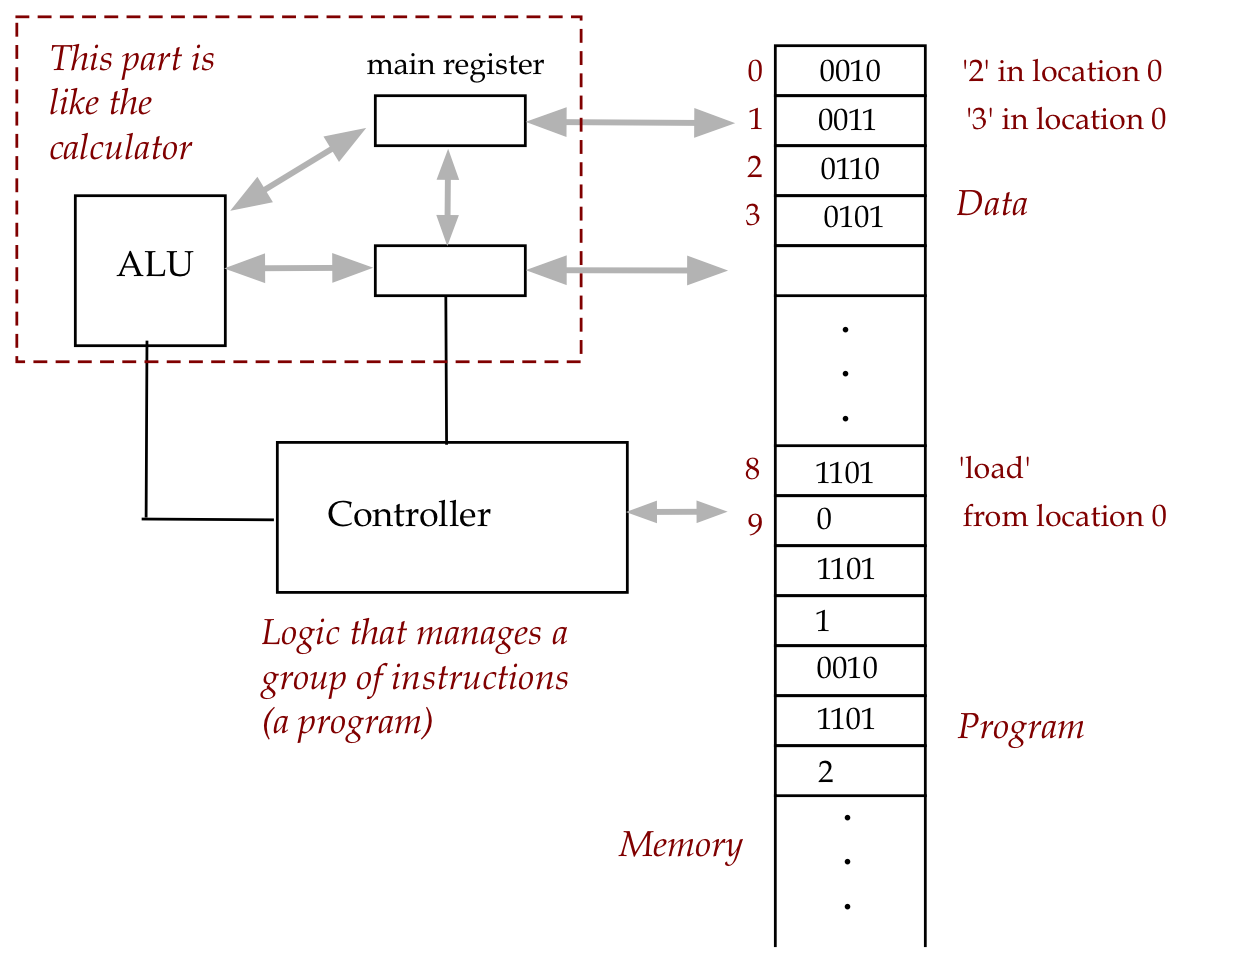
\includegraphics[width=4in]{notes/figs/n08/03program.png}
        \caption{1950s computer}
        \label{fig:03program}
    \end{figure}
    
    This is now a whole level of additional power and complexity. One can write programs that execute in the same hardware that "calculates". The programs themselves can be long and feature loops, conditionals (if-then's) and other features. Within $20+$ years after the earliest machines, the earliest abstractions of algorithms began to appear, for example:
    
    Method: quickSort (data, L, R)\\
    Input: data - an array of size $n$ with a subrange specified by $I$ and R\\
    1. if $\mathrm{L} \geq \mathrm{R}$\\
    2. return \\
    3. endif \\
    // Partition the array and position partition element correctly.\\
    4. $p=$ partition (data, L, R) \\
    5. quickSortRecursive (data, L, p-1) // Sort left side \\
    6. quicksortRecursive (data, $p+1, R$ ) // Sort right side \\
    
    The astonishing power of such abstraction has led to the modern world of computing. Many of these high-level abstractions (like recursion) are hard to understand from the "circuit level view". The contrast: Currently, quantum computing is in the 1940's era of classical computing: The focus is on getting circuits to work at scale. It's not even clear that the standard circuit model will dominate: Other proposed architectures apply measurements along the way. Yet others use mostly measurements. And more exotic approaches feature continuous, as opposed to discrete, optimization. At a later time, one anticipates some integration into classical hardware referenced in Figure \ref{fig:04program2}.
    
    \begin{figure}
        \centering
        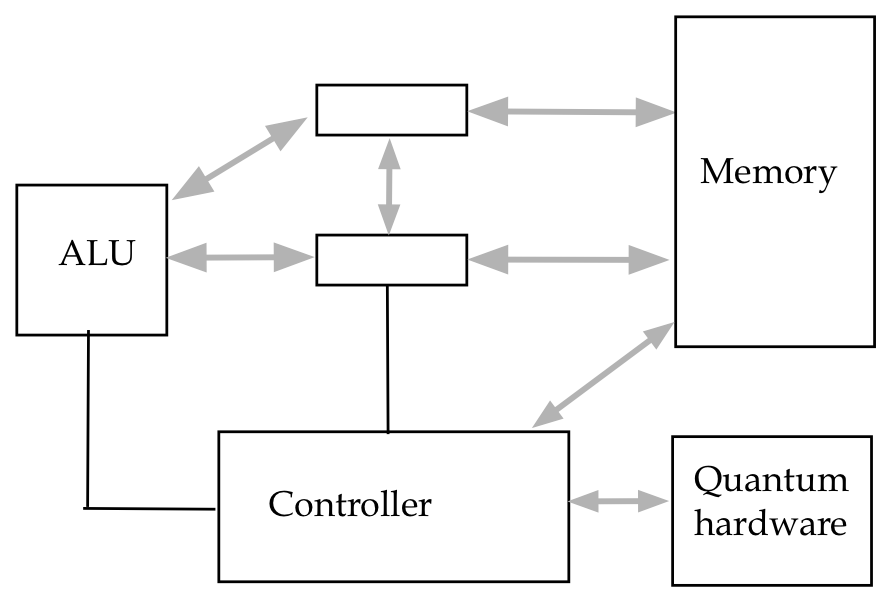
\includegraphics[width=4in]{notes/figs/n08/04program2.png}
        \caption{integration into classical hardware}
        \label{fig:04program2}
    \end{figure}
    
    What one hopes for the future (your generation): Powerful high-level abstractions akin to classical programming. Questions that need answers: Which circuit model is best? What high-level abstractions are useful? How do these abstractions integrate classical and quantum? How can the circuit part be automated? What problems and algorithms are demonstrably (and practically) faster on quantum hardware? What new and unexpected uses might arise from quantum computing? The next steps for us: Learn about commonly used gates (this module). Learn to use the drawing conventions, Dirac and matrix representations. Systematically build larger circuits (next module)

\subsection{Commonly used 1-qubit gates: Pauli and exponentiated-Pauli gates}

    Let's begin with the four Pauli gates shown in Figure \ref{fig:05gate1}.
    
    \begin{figure}
        \centering
        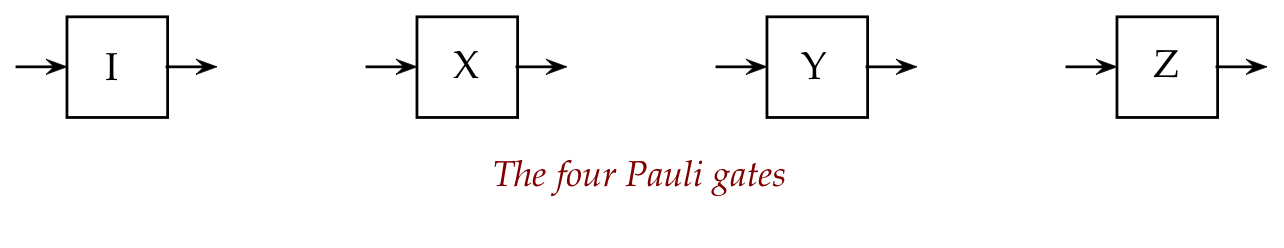
\includegraphics[width=4in]{notes/figs/n08/05gate1.png}
        \caption{four Pauli gates}
        \label{fig:05gate1}
    \end{figure}
    
    In matrix and Dirac form:
    
    $$
    \begin{aligned}
    &I=|0\rangle\langle 0|+| 1\rangle\langle 1| \quad=\left[\begin{array}{ll}
    1 & 0 \\
    0 & 1
    \end{array}\right]\\
    &X=|0\rangle\langle 1|+| 1\rangle\langle 0| \quad=\left[\begin{array}{ll}
    0 & 1 \\
    1 & 0
    \end{array}\right]\\
    &Y=-i|0\rangle\langle 1|+i| 1\rangle\langle 0|=\left[\begin{array}{cc}
    0 & -i \\
    i & 0
    \end{array}\right]\\
    &Z=|0\rangle\langle 0|-| 1\rangle\langle 1|=\left[\begin{array}{cc}
    1 & 0 \\
    0 & -1
    \end{array}\right]
    \end{aligned}
    $$
    
    The action of $X$ on a general qubit:
    
    $$
    X(\alpha|0\rangle+\beta|1\rangle)=(|0\rangle\langle 1|+| 1\rangle\langle 0|)(\alpha|0\rangle+\beta|1\rangle)=\beta|0\rangle+\alpha|1\rangle
    $$
    
    Note: $X$ switches the standard basis vectors:
    
    $$
    \begin{aligned}
    &X|0\rangle=|1\rangle \\
    &X|1\rangle=|0\rangle
    \end{aligned}
    $$
    
    But not the Hadamard basis vectors:
    
    $$
    \begin{array}{ll}
    X|+\rangle= & |+\rangle \\
    X|-\rangle= & -|-\rangle
    \end{array}
    $$
    
    Note:
    
    $$
    -|-\rangle=e^{i \pi}|-\rangle
    $$
    
    and so $|-\rangle$ and $-|-\rangle$ are the same qubit state (global-phase equivalent). Next, consider $Z$ :
    
    $$
    \begin{array}{rlr}
    Z(\alpha|0\rangle+\beta|1\rangle) & =(|0\rangle\langle 0|-| 1\rangle\langle 1|)(\alpha|0\rangle+\beta|1\rangle) & \\
    & =\alpha|0\rangle-\beta|1\rangle & =\alpha|0\rangle+e^{i \pi} \beta|1\rangle
    \end{array}
    $$
    
    which changes the sign of the $|1\rangle$ component. Some special cases for $Z$:
    
    $$
    \begin{aligned}
    Z|0\rangle &=|0\rangle \\
    Z|1\rangle &=e^{i \pi}|1\rangle \\
    Z|+\rangle &=|-\rangle \\
    Z|-\rangle &=|+\rangle
    \end{aligned}
    $$
    
    Thus, $Z$ switches the Hadamard vectors, but not the $|0\rangle,|1\rangle$. Pauli gates are named in honor of Wolfgang Pauli, one of the early major contributors to the development of quantum mechanics.
    
    Useful properties: Each Pauli gate is both unitary and Hermitian. The square of a Pauli gate is the identity:
    
    $$
    I^{2}=X^{2}=Y^{2}=Z^{2}=I
    $$
    
    Pairwise identities:
    
    $$
    \begin{aligned}
    &X Y=-Y X=i Z \\
    &Y Z=-Z Y=i X \\
    &Z X=-X Z=i Y
    \end{aligned}
    $$
    
\subsection{Commonly used 1-qubit gates: exponentiated-Pauli gates}

    It turns out that some exponentiated Pauli gates like $\sqrt{Z}=Z^{\frac{1}{2}}$ are unitary and useful. Let's examine how to calculate the matrices: Recall this useful result (Module 4): if $A^{2}=I$ then
    
    $$
    e^{i \theta A}=I \cos \theta+i A \sin \theta
    $$
    
    Then, with $A=X$
    
    $$
    \begin{aligned}
    e^{\frac{-i \theta}{2} X} &=I \cos \frac{-\theta}{2}+i X \sin \frac{-\theta}{2} \\
    &=\cos \frac{\theta}{2}\left[\begin{array}{ll}
    1 & 0 \\
    0 & 1
    \end{array}\right]-\sin \frac{\theta}{2}\left[\begin{array}{ll}
    0 & i \\
    i & 0
    \end{array}\right] \\
    &=\left[\begin{array}{cc}
    \cos \frac{\theta}{2} & -i \sin \frac{\theta}{2} \\
    -i \sin \frac{\theta}{2} & \cos \frac{\theta}{2}
    \end{array}\right]
    \end{aligned}
    $$
    
    This is given the special name $R_{X}(\theta)$. One can similarly exponentiate $Y, Z$ with the same half-angle. Let's write these down:
    
    $$
    \begin{aligned}
    &R_{X}(\theta)=e^{\frac{-i \theta}{2} X}=\left[\begin{array}{cc}
    \cos \frac{\theta}{2} & -i \sin \frac{\theta}{2} \\
    -i \sin \frac{\theta}{2} & \cos \frac{\theta}{2}
    \end{array}\right] \\
    &R_{Y}(\theta)=e^{\frac{-i \theta}{2} Y}=\left[\begin{array}{cc}
    \cos \frac{\theta}{2} & -\sin \frac{\theta}{2} \\
    \sin \frac{\theta}{2} & \cos \frac{\theta}{2}
    \end{array}\right] \\
    &R_{Z}(\theta)=e^{\frac{-i \theta}{2} Z}=\left[\begin{array}{cc}
    e^{\frac{-i \theta}{2}} & 0 \\
    0 & e^{\frac{i \theta}{2}}
    \end{array}\right]
    \end{aligned}
    $$
    
    You might be curious: why use the half-angle in the definition? There is a geometric object called the Bloch sphere that is sometimes used to visual actions on a single qubit. This is an artificial geometry that does not correspond to anything in the real world. It turns out that the matrices above correspond to $\theta$-rotations of the axes of this sphere. This is why the three matrices are sometimes called rotation matrices. They perform rotations in the fictional Bloch sphere world. The exponential notation makes it obvious that
    
    $$
    \begin{aligned}
    &R_{X}\left(\theta_{1}+\theta_{2}\right)=R_{X}\left(\theta_{1}\right) R_{X}\left(\theta_{2}\right) \\
    &R_{Y}\left(\theta_{1}+\theta_{2}\right)=R_{Y}\left(\theta_{1}\right) R_{Y}\left(\theta_{2}\right) \\
    &R_{Z}\left(\theta_{1}+\theta_{2}\right)=R_{Z}\left(\theta_{1}\right) R_{Z}\left(\theta_{2}\right)
    \end{aligned}
    $$
    
    For example:
    
    $$
    R_{X}\left(\theta_{1}\right) R_{X}\left(\theta_{2}\right)=e^{\frac{-i \theta_{1}}{2} X} e^{\frac{-i \theta_{2}}{2} X}=e^{\frac{\left.-i \theta_{1}+\theta_{2}\right)}{2} X}=R_{X}\left(\theta_{1}+\theta_{2}\right)
    $$
    
    All three are unitary. For example:
    
    $$
    \begin{aligned}
    R_{X}(\theta)^{\dagger} R_{X}(\theta) &=\left[\begin{array}{cc}
    \cos \frac{\theta}{2} & i \sin \frac{\theta}{2} \\
    i \sin \frac{\theta}{2} & \cos \frac{\theta}{2}
    \end{array}\right]\left[\begin{array}{cc}
    \cos \frac{\theta}{2} & -i \sin \frac{\theta}{2} \\
    -i \sin \frac{\theta}{2} & \cos \frac{\theta}{2}
    \end{array}\right] \\
    &=\left[\begin{array}{cc}
    \cos ^{2} \frac{\theta}{2}+\sin ^{2} \frac{\theta}{2} & 0 \\
    0 & \cos ^{2} \frac{\theta}{2}+\sin ^{2} \frac{\theta}{2}
    \end{array}\right] \\
    &=I
    \end{aligned}
    $$
    
    Three special cases: Recall:
    
    $$
    R_{Z}(\theta)=e^{\frac{-i \theta}{2} Z}=\left[\begin{array}{cc}
    e^{\frac{-i \theta}{2}} & 0 \\
    0 & e^{\frac{i \theta}{2}}
    \end{array}\right]
    $$
    
    With $\alpha=-\frac{\theta}{2}$, we can write
    
    $$
    \begin{aligned}
    e^{i \alpha Z}=& {\left[\begin{array}{cc}
    e^{i \alpha} & 0 \\
    0 & e^{-i \alpha}
    \end{array}\right] } \\
    & \triangleq T(\alpha)
    \end{aligned}
    $$
    
    We'll call this the $T(\alpha)$ gate, following the textbook. Consider a similar substitution $\beta=-\frac{\theta}{2}$ in
    
    $$
    R_{Y}(\theta)=e^{\frac{-i \theta}{2} Y}=\left[\begin{array}{cc}
    \cos \frac{\theta}{2} & -\sin \frac{\theta}{2} \\
    \sin \frac{\theta}{2} & \cos \frac{\theta}{2}
    \end{array}\right]
    $$
    
    This gives us
    
    $$
    \begin{gathered}
    e^{i \beta Y}=\left[\begin{array}{cc}
    \cos \beta & \sin \beta \\
    -\sin \beta & \cos \beta
    \end{array}\right] \\
    \triangleq R(\beta)
    \end{gathered}
    $$
    
    It's slightly confusing but we'll call this gate $R(\beta)$ in keeping with the textbook. Finally, substitute $A=I$ in
    
    $$
    e^{i \theta A}=I \cos \theta+i A \sin \theta
    $$
    
    to get
    
    $$
    e^{i \theta I}=I \cos \theta+i I \sin \theta=e^{i \theta} I
    $$
    
    The gate
    
    $$
    K(\delta)=e^{i \delta} I=\left[\begin{array}{cc}
    e^{i \delta} & 0 \\
    0 & e^{i \delta}
    \end{array}\right]
    $$
    
    changes global-phase, which is occasionally useful in simplification. For example:
    
    $$
    K(\delta)(\alpha|0\rangle+\beta|1\rangle)=\left[\begin{array}{cc}
    e^{i \delta} & 0 \\
    0 & e^{i \delta}
    \end{array}\right]\left[\begin{array}{c}
    \alpha \\
    \beta
    \end{array}\right]=e^{i \delta}\left[\begin{array}{l}
    \alpha \\
    \beta
    \end{array}\right]=e^{i \delta}(\alpha|0\rangle+\beta|1\rangle)
    $$
    
    In summary:
    $$
    \begin{aligned}
    T(\alpha) &=\left[\begin{array}{cc}
    e^{i \alpha} & 0 \\
    0 & e^{-i \alpha}
    \end{array}\right] \\
    R(\beta) &=\left[\begin{array}{cc}
    \cos \beta & \sin \beta \\
    -\sin \beta & \cos \beta
    \end{array}\right] \\
    K(\delta) &=\left[\begin{array}{cc}
    e^{i \delta} & 0 \\
    0 & e^{i \delta}
    \end{array}\right]
    \end{aligned}
    $$
    
    Clearly, from the exponentiated origin,
    
    $$
    \begin{aligned}
    T\left(\alpha_{1}+\alpha_{2}\right) &=T\left(\alpha_{1}\right) T\left(\alpha_{2}\right) \\
    R\left(\beta_{1}+\beta_{2}\right) &=R\left(\beta_{1}\right) R\left(\beta_{2}\right) \\
    K\left(\delta_{1}+\delta_{2}\right) &=K\left(\delta_{1}\right) K\left(\delta_{2}\right)
    \end{aligned}
    $$
    
    And
    
    $$
    \begin{aligned}
    T(0) &=\left[\begin{array}{cc}
    e^{0} & 0 \\
    0 & e^{0}
    \end{array}\right]=I \\
    R(0) &=\left[\begin{array}{cc}
    \cos 0 & \sin 0 \\
    -\sin 0 & \cos 0
    \end{array}\right] \\
    &=I
    \end{aligned}
    $$
    
    And, of course, all three are unitary. For example:
    
    $$
    \begin{aligned}
    K(\delta)^{\dagger} K(\delta) &=\left(e^{i \delta} I\right)^{\dagger}\left(e^{i \delta} I\right) \\
    &=\left(e^{i \delta}\right)^{*} I e^{i \delta} I \\
    &=e^{-i \delta} I e^{i \delta} I \\
    &=I
    \end{aligned}
    $$
    
\subsection{Commonly used 1-qubit gates: powered Pauli gates}

    First, let's point out a consequence of global-phase equivalence: Recall what this means: Two vectors $|\psi\rangle$ and $|\phi\rangle$ are global-phase equivalent if
    
    $$
    |\psi\rangle=e^{i \theta}|\phi\rangle
    $$
    
    for some $\theta$. Both vectors then represent the same qubit state. Remember: measurement cannot tell them apart, because the $e^{i \theta}$ magnitude does not change probabilities. For example, in
    
    $$
    e^{i \theta} \alpha|0\rangle+e^{i \theta} \beta|1\rangle
    $$
    
    the probability for $|0\rangle$ is
    
    $$
    \left|e^{i \theta} \alpha\right|^{2}=\left|e^{i \theta}\right|^{2}|\alpha|^{2}=|\alpha|^{2}
    $$
    
    This means if
    
    $$
    |\phi\rangle=U|\psi\rangle
    $$
    
    for any unitary $U$ then
    
    $$
    e^{i \theta}|\phi\rangle=\left(e^{i \theta} U\right)|\psi\rangle
    $$
    
    That is, $U$ and $e^{i \theta} U$ result in two global-phase equivalent vectors. And so, one can drop or factor out $e^{i \theta}$ from any unitary $e^{i \theta} U$. Now let's turn to fractional powers of the Pauli operators. The special property $Z^{2}=I$ makes it possible to easily derive $Z^{\frac{1}{2}}$ and $Z^{\frac{1}{4}}$: First, observe that
    
    $$
    e^{-i \frac{\pi}{2} Z}=\left[\begin{array}{cc}
    e^{-\frac{\pi}{2}} & 0 \\
    0 & e^{\frac{\pi}{2}}
    \end{array}\right]=\left[\begin{array}{cc}
    -i & 0 \\
    0 & i
    \end{array}\right]=-i Z
    $$
    
    Next because $I^{2}=I$, the $A^{2}=I$ exponentiation property gives us
    
    $$
    e^{i \theta I}=I \cos \theta+i I \sin \theta
    $$
    
    and so
    
    $$
    e^{i \frac{\pi}{2} I}=i I
    $$
    
    Combining the two results:
    
    $$
    e^{-i Z \frac{\pi}{2}} e^{i I \frac{\pi}{2}}=(-i Z)(i I)=Z
    $$
    
    Now raise both sides to the power $t$ :
    
    $$
    Z^{t}=e^{-i Z t \frac{\pi}{2}} e^{i I t \frac{\pi}{2}}
    $$
    
    Thus, we have a way to compute fractional powers like $Z^{\frac{1}{2}}$ and $Z^{\frac{1}{4}}$. A further simplification ensues from
    
    $$
    \begin{aligned}
    e^{i I t \frac{\pi}{2}} &=\left(e^{i I \frac{\pi}{2}}\right)^{t} \\
    &=(i I)^{t} \\
    &=\left(e^{i \frac{\pi}{2}} I\right)^{t} \\
    &=\left(e^{i \frac{\pi}{2}}\right)^{t} I^{t} \\
    &=e^{i t \frac{\pi}{2}} I
    \end{aligned}
    $$
    
    Then,
    
    $$
    \begin{aligned}
    Z^{t} &=e^{-i Z t \frac{\pi}{2}} e^{i l t \frac{\pi}{2}} \\
    &=R_{Z}(\pi t) e^{i t \frac{\pi}{2}} I \\
    &=e^{i t \frac{\pi}{2}} R_{Z}(\pi t) I \\
    &=e^{i t \frac{\pi}{2}} R_{Z}(\pi t)
    \end{aligned}
    $$
    
    With $t=\frac{1}{2}$
    
    $$
    \begin{aligned}
    Z^{\frac{1}{2}} &=e^{i \frac{\pi}{4}} R_{Z}\left(\frac{\pi}{2}\right) \\
    &=e^{i \frac{\pi}{4}}\left[\begin{array}{c}
    e^{-i \frac{\pi}{4}} \\
    0
    \end{array}\right.\\
    &=\left[\begin{array}{cc}
    1 & 0 \\
    0 & e^{i \frac{\pi}{2}}
    \end{array}\right] \\
    &=\left[\begin{array}{ll}
    1 & 0 \\
    0 & i
    \end{array}\right] \\
    & \triangleq \text { S-gate }
    \end{aligned}
    $$
    
    Similarly, with $t=\frac{1}{4}$, we get
    
    $$
    \begin{aligned}
    Z^{\frac{1}{4}} &=\left[\begin{array}{cc}
    1 & 0 \\
    0 & e^{i \frac{\pi}{4}}
    \end{array}\right] \\
    & \triangleq \text { T-gate }
    \end{aligned}
    $$
    
    For general $t=\theta$,
    
    $$
    \begin{aligned}
    Z^{\theta} &=e^{i \theta \frac{\pi}{2}} R_{Z}(\pi \theta) \\
    &=e^{i \theta \frac{\pi}{2}}\left[\begin{array}{cc}
    e^{-i \theta \frac{\pi}{2}} & 0 \\
    0 & e^{i \theta \frac{\pi}{2}}
    \end{array}\right] \\
    &=\left[\begin{array}{cc}
    1 & 0 \\
    0 & e^{i \pi \theta}
    \end{array}\right]
    \end{aligned}
    $$
    
    When substituting $t=\frac{\theta}{\pi}$ :
    
    $$
    \begin{aligned}
    Z^{\frac{\theta}{\pi}} &=\left[\begin{array}{cc}
    1 & 0 \\
    0 & e^{i \theta}
    \end{array}\right] \\
    & \triangleq P(\theta) \text {-gate }
    \end{aligned}
    $$
    
    This achieves a change in relative phase in a qubit:
    
    $$
    P(\theta)(\alpha|0\rangle+\beta|1\rangle)=\left[\begin{array}{cc}
    1 & 0 \\
    0 & e^{i \theta}
    \end{array}\right]\left[\begin{array}{c}
    \alpha \\
    \beta
    \end{array}\right]=\left[\begin{array}{c}
    \alpha \\
    e^{i \theta} \beta
    \end{array}\right]=\alpha|0\rangle+e^{i \theta} \beta|1\rangle
    $$
    
    Note: the vectors
    
    $$
    \alpha|0\rangle+\beta|1\rangle
    $$
    
    and
    
    $$
    \alpha|0\rangle+e^{i \pi \theta} \beta|1\rangle
    $$
    
    do not represent the same qubit state. To summarize:
    
    $$
    \begin{aligned}
    S &=\left[\begin{array}{ll}
    1 & 0 \\
    0 & i
    \end{array}\right] \\
    T &=\left[\begin{array}{ll}
    1 & 0 \\
    0 & e^{i \frac{\pi}{4}}
    \end{array}\right] \\
    P(\theta) &=\left[\begin{array}{cc}
    1 & 0 \\
    0 & e^{i \theta}
    \end{array}\right]
    \end{aligned}
    $$
    
    All are unitary. For example:
    
    $$
    S^{\dagger} S=\left[\begin{array}{cc}
    1 & 0 \\
    0 & -i
    \end{array}\right]\left[\begin{array}{ll}
    1 & 0 \\
    0 & i
    \end{array}\right]=I
    $$
    
    Finally, let's list the important powers for convenience:
    
    $$
    \begin{aligned}
    X^{\frac{1}{2}} &=\frac{1}{2}\left[\begin{array}{cc}
    1+i & 1-i \\
    1-i & 1+i
    \end{array}\right] \\
    Y^{\frac{1}{2}} &=\frac{e^{i \frac{\pi}{4}}}{\sqrt{2}}\left[\begin{array}{cc}
    1 & -1 \\
    1 & 1
    \end{array}\right] \\
    Z^{\frac{1}{2}} &=\left[\begin{array}{cc}
    1 & 0 \\
    0 & i
    \end{array}\right] \\
    Z^{\frac{1}{4}} &=\left[\begin{array}{cc}
    1 & 0 \\
    0 & e^{i \frac{\pi}{4}}
    \end{array}\right] \\
    Z^{\frac{\theta}{\pi}} &=\left[\begin{array}{cc}
    1 & 0 \\
    0 & e^{i \theta}
    \end{array}\right]
    \end{aligned}
    $$

\subsection{Commonly used 1-qubit gates: Hadamard}

    We have already introduced the Hadamard, but let's include it here for completeness, and also add some new properties: reference Figure \ref{fig:06gate5}.
    
    \begin{figure}
        \centering
        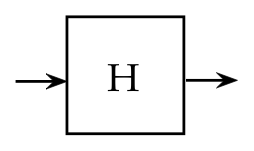
\includegraphics[width=3in]{notes/figs/n08/06gate5.png}
        \caption{Hadamard gate}
        \label{fig:06gate5}
    \end{figure}
    
    The Hadamard gate is
    
    $$
    H=\left[\begin{array}{cc}
    \frac{1}{\sqrt{2}} & \frac{1}{\sqrt{2}} \\
    \frac{1}{\sqrt{2}} & -\frac{1}{\sqrt{2}}
    \end{array}\right]=\frac{1}{\sqrt{2}}\left[\begin{array}{cc}
    1 & 1 \\
    1 & -1
    \end{array}\right]
    $$
    
    It converts back and forth between standard and H-basis vectors:
    
    $$
    \begin{aligned}
    H|0\rangle &=|+\rangle \\
    H|1\rangle &=|-\rangle \\
    H|+\rangle &=|0\rangle \\
    H|-\rangle &=|1\rangle
    \end{aligned}
    $$
    
    And we've seen its fundamental role in creating n-qubit superpositions as referenced in Figure \ref{fig:07gate6}.
    
    \begin{figure}
        \centering
        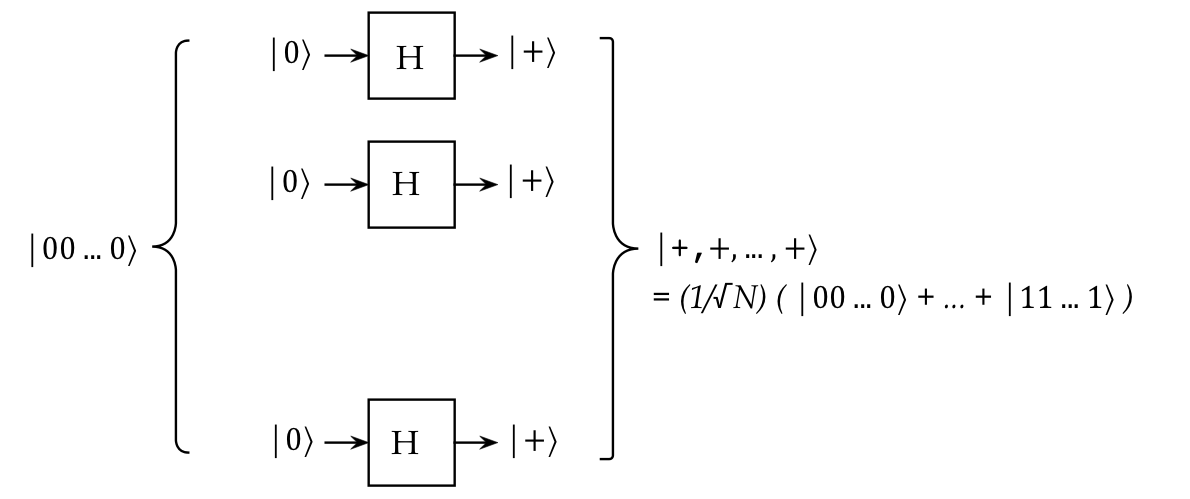
\includegraphics[width=5in]{notes/figs/n08/07gate6.png}
        \caption{creating n-qubit superpositions}
        \label{fig:07gate6}
    \end{figure}
    
    Here, for the n-qubit case:
    
    $$
    (H \otimes H \otimes \ldots \otimes H)|00 \ldots 0\rangle=\frac{1}{\sqrt{N}}(|00 \ldots 0\rangle+\ldots+|11 \ldots 1\rangle)
    $$
    
    where $N=2^{n}$. Observe: We've performed $n$ operations above (a polynomial number), in parallel. And obtained an exponential number of vectors in the superposition: $N=2^{n}$. We often use the decimal version of the standard basis
    
    $$
    \begin{aligned}
        |0\rangle & =|00 \ldots 0\rangle\\
        |1\rangle & =|00 \ldots 1\rangle\\
        |2\rangle & =|0 \ldots 10\rangle\\
        |3\rangle & =|0 \ldots 11\rangle\\
                & \cdots \\
        |N-1\rangle & =|1 \ldots 11\rangle
    \end{aligned}
    $$
    
    and write
    
    $$
    \begin{aligned}
    \frac{1}{\sqrt{N}}(|00 \ldots 0\rangle+\ldots+|11 \ldots 1\rangle) &=\frac{1}{\sqrt{N}}(|0\rangle+|1\rangle \ldots+|N-1\rangle) \\
    &=\frac{1}{\sqrt{N}} \sum_{i=0}^{N-1}|i\rangle
    \end{aligned}
    $$
    
    The Hadamard with other 1-qubit gates: The following identities are easily established:
    
    $$
    \begin{aligned}
    H X H &=Z \\
    H Z H &=X \\
    H Y H &=-Y \\
    H R_{X}(\theta) H &=R_{Z}(\theta) \\
    H R_{Z}(\theta) H &=R_{X}(\theta) \\
    H R_{Y}(\theta) H &=R_{Y}(-\theta)
    \end{aligned}
    $$
    
    For example reference \fig{fig:08gate7}.
    
    \begin{figure}
        \centering
        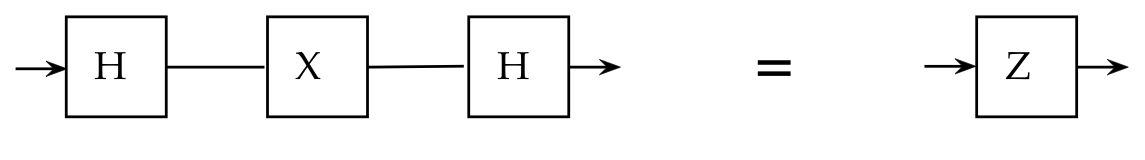
\includegraphics[width=5in]{notes/figs/n08/08gate7.png}
        \caption{$H X H$}
        \label{fig:08gate7}
    \end{figure}
    
    $$
    \begin{aligned}
    H X H &=\frac{1}{\sqrt{2}}\left[\begin{array}{cc}
    1 & 1 \\
    1 & -1
    \end{array}\right]\left[\begin{array}{cc}
    0 & 1 \\
    1 & 0
    \end{array}\right] \frac{1}{\sqrt{2}}\left[\begin{array}{cc}
    1 & 1 \\
    1 & -1
    \end{array}\right] \\
    &=\frac{1}{2}\left[\begin{array}{cc}
    1 & 1 \\
    1 & -1
    \end{array}\right]\left[\begin{array}{cc}
    1 & -1 \\
    1 & 1
    \end{array}\right] \\
    &=\frac{1}{2}\left[\begin{array}{cc}
    2 & 0 \\
    0 & -2
    \end{array}\right] \\
    &=Z
    \end{aligned}
    $$
    
    Another example reference \ref{fig:09gate8}.
    
    \begin{figure}
        \centering
        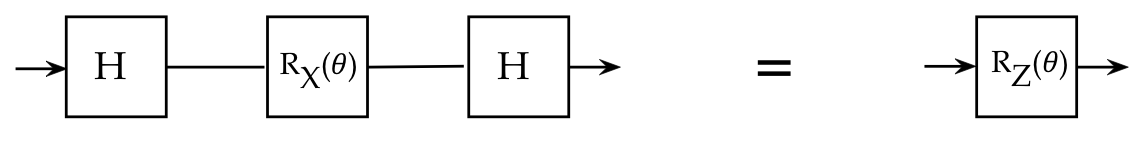
\includegraphics[width=5in]{notes/figs/n08/09gate8.png}
        \caption{$H R_X(\theta) H$}
        \label{fig:09gate8}
    \end{figure}
    
    $$
    \begin{aligned}
    H R_{X}(\theta) H &=\frac{1}{\sqrt{2}}\left[\begin{array}{cc}
    1 & 1 \\
    1 & -1
    \end{array}\right]\left[\begin{array}{cc}
    \cos \frac{\theta}{2} & -i \sin \frac{\theta}{2} \\
    -i \sin \frac{\theta}{2} & \cos \frac{\theta}{2}
    \end{array}\right] \frac{1}{\sqrt{2}}\left[\begin{array}{cc}
    1 & 1 \\
    1 & -1
    \end{array}\right] \\
    &=\frac{1}{2}\left[\begin{array}{cc}
    1 & 1 \\
    1 & -1
    \end{array}\right]\left[\begin{array}{cc}
    e^{-i \frac{\theta}{2}} & e^{i \frac{\theta}{2}} \\
    e^{-i \frac{\theta}{2}} & -e^{i \frac{\theta}{2}}
    \end{array}\right] \\
    &=\frac{1}{2}\left[\begin{array}{cc}
    2 e^{-i \frac{\theta}{2}} & 0 \\
    0 & -2 e^{i \frac{\theta}{2}}
    \end{array}\right] \\
    &=R_{Z}(\theta)
    \end{aligned}
    $$

\subsection{Summary of important 1-qubit gates}

    For convenience, let's list all the gates so far. The main Pauli gates referenced in Figure \ref{fig:10gate1}
    
    \begin{figure}
        \centering
        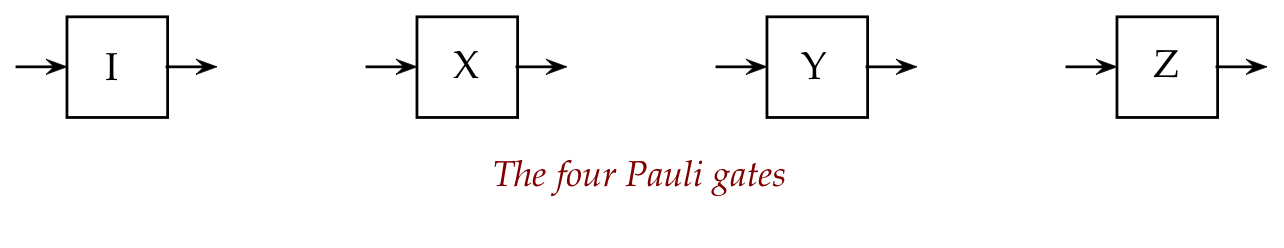
\includegraphics[width=5in]{notes/figs/n08/10gate1.png}
        \caption{The four Pauli gates}
        \label{fig:10gate1}
    \end{figure}
    
    $$
    \begin{aligned}
    I &=\left[\begin{array}{ll}
    1 & 0 \\
    0 & 1
    \end{array}\right] \\
    X &=\left[\begin{array}{ll}
    0 & 1 \\
    1 & 0
    \end{array}\right] \\
    Y &=\left[\begin{array}{cc}
    0 & -i \\
    i & 0
    \end{array}\right] \\
    Z &=\left[\begin{array}{cc}
    1 & 0 \\
    0 & -1
    \end{array}\right]
    \end{aligned}
    $$
    
    The three rotation gates $R_{X}(\theta), R_{Y}(\theta), R_{Z}(\theta)$ shown in Figure \ref{fig:11gate2}.
    
    \begin{figure}
        \centering
        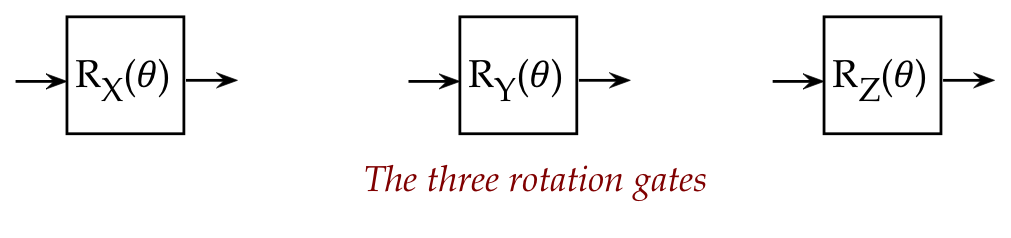
\includegraphics[width=5in]{notes/figs/n08/11gate2.png}
        \caption{Three rotation gates}
        \label{fig:11gate2}
    \end{figure}
    
    $$
    \begin{aligned}
    &R_{X}(\theta)=e^{\frac{-i \theta}{2} X}=\left[\begin{array}{cc}
    \cos \frac{\theta}{2} & -i \sin \frac{\theta}{2} \\
    -i \sin \frac{\theta}{2} & \cos \frac{\theta}{2}
    \end{array}\right] \\
    &R_{Y}(\theta)=e^{\frac{-i \theta}{2} Y}=\left[\begin{array}{cc}
    \cos \frac{\theta}{2} & -\sin \frac{\theta}{2} \\
    \sin \frac{\theta}{2} & \cos \frac{\theta}{2}
    \end{array}\right] \\
    &R_{Z}(\theta)=e^{\frac{-i \theta}{2} Z}=\left[\begin{array}{cc}
    e^{\frac{-i \theta}{2}} & 0 \\
    0 & e^{\frac{i \theta}{2}}
    \end{array}\right]
    \end{aligned}
    $$
    
    The $T(\alpha), R(\beta)$ and $K(\delta)$ gates shown in Figure \ref{fig:12gate3}.
    
    \begin{figure}
        \centering
        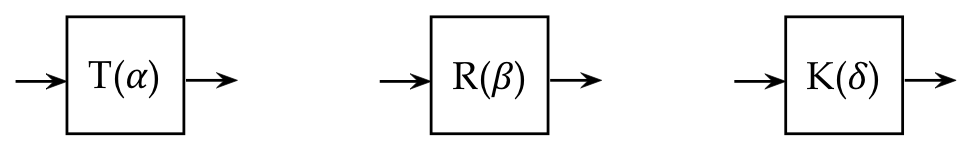
\includegraphics[width=5in]{notes/figs/n08/12gate3.png}
        \caption{$T(\alpha), R(\beta)$ and $K(\delta)$}
        \label{fig:12gate3}
    \end{figure}
    
    $$
    \begin{aligned}
    &T(\alpha)=e^{i \alpha Z}=\left[\begin{array}{cc}
    e^{i \alpha} & 0 \\
    0 & e^{-i \alpha}
    \end{array}\right] \\
    &R(\beta)=e^{i \beta Y}=\left[\begin{array}{cc}
    \cos \beta & \sin \beta \\
    -\sin \beta & \cos \beta
    \end{array}\right] \\
    &K(\delta)=e^{i \delta I}=\left[\begin{array}{cc}
    e^{i \delta} & 0 \\
    0 & e^{i \delta}
    \end{array}\right]
    \end{aligned}
    $$
    
    The $T(\alpha), R(\beta)$ and $K(\delta)$ gates shown in Figure \ref{fig:13gate4}.
    
    \begin{figure}
        \centering
        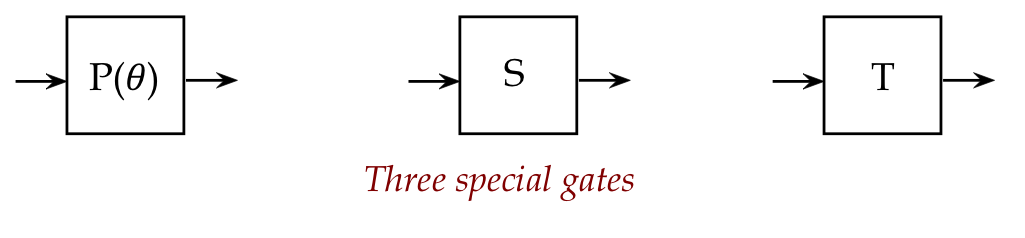
\includegraphics[width=5in]{notes/figs/n08/13gate4.png}
        \caption{Three special gates}
        \label{fig:13gate4}
    \end{figure}
    
    $$
    \begin{aligned}
    P(\theta) &=Z^{\frac{\theta}{\pi}}=\left[\begin{array}{cc}
    1 & 0 \\
    0 & e^{i \pi \theta}
    \end{array}\right] \\
    S &=Z^{\frac{1}{2}}=\left[\begin{array}{ll}
    1 & 0 \\
    0 & i
    \end{array}\right] \\
    T &=Z^{\frac{1}{4}}=\left[\begin{array}{cc}
    1 & 0 \\
    0 & e^{i \frac{\pi}{4}}
    \end{array}\right]
    \end{aligned}
    $$
    
    And of course the Hadamard shown in Figure \ref{fig:14gate5}.
    
    \begin{figure}
        \centering
        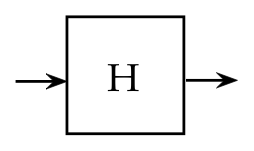
\includegraphics[width=2in]{notes/figs/n08/14gate5.png}
        \caption{Hadamard}
        \label{fig:14gate5}
    \end{figure}
    
    $$
    H=\left[\begin{array}{cc}
    \frac{1}{\sqrt{2}} & \frac{1}{\sqrt{2}} \\
    \frac{1}{\sqrt{2}} & -\frac{1}{\sqrt{2}}
    \end{array}\right]=\frac{1}{\sqrt{2}}\left[\begin{array}{cc}
    1 & 1 \\
    1 & -1
    \end{array}\right]
    $$

\subsection{An example with 1-qubit gates}

    Let's analyze an example circuit in few different ways shown in Figure \ref{fig:15circuitexample1}.
    
    \begin{figure}
        \centering
        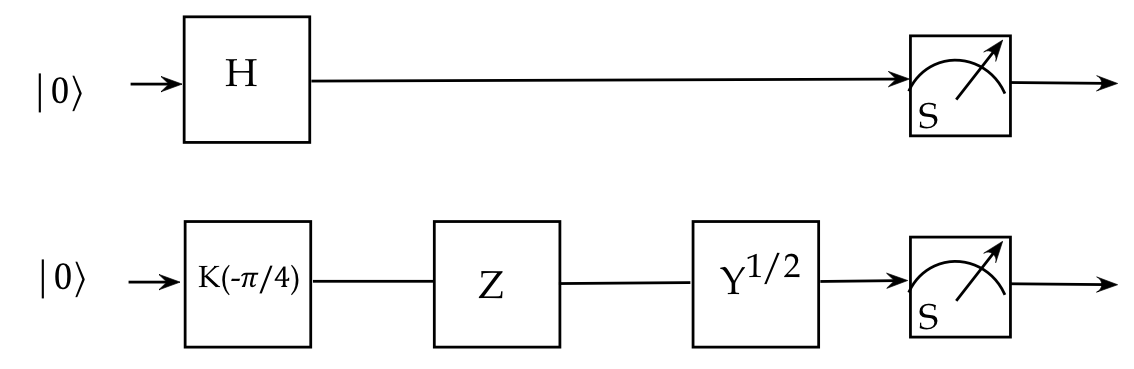
\includegraphics[width=5in]{notes/figs/n08/15circuitexample1.png}
        \caption{Example circuit}
        \label{fig:15circuitexample1}
    \end{figure}
    
    where
    
    $$
    Y^{\frac{1}{2}}=\frac{e^{i \frac{\pi}{4}}}{\sqrt{2}}\left[\begin{array}{cc}
    1 & -1 \\
    1 & 1
    \end{array}\right]
    $$
    
    First, let's infer the stages and implied tensored operators shown in Figure \ref{fig:16circuitexample2}.
    
    \begin{figure}
        \centering
        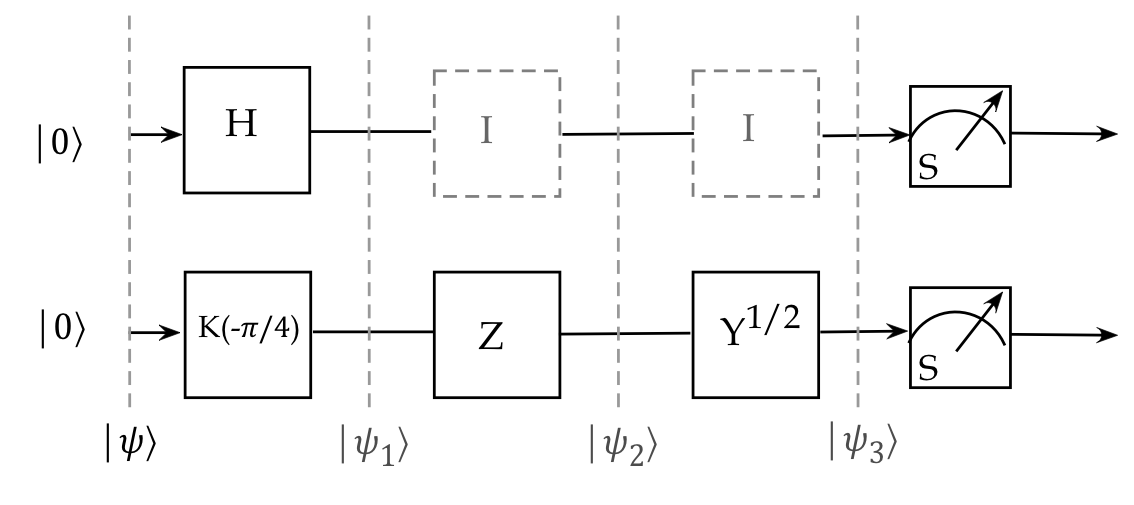
\includegraphics[width=5in]{notes/figs/n08/16circuitexample2.png}
        \caption{Implied tensored operators}
        \label{fig:16circuitexample2}
    \end{figure}
    
    We see that the input state is $|\psi\rangle=|00\rangle$. The first 2-qubit unitary is: $H \otimes K\left(-\frac{\pi}{4}\right)$, resulting in state $\left|\psi_{1}\right\rangle$ :
    
    $$
    \left|\psi_{1}\right\rangle=\left(H \otimes K\left(-\frac{\pi}{4}\right)\right)|\psi\rangle
    $$
    
    After this, the 2 -qubit unitary $I \otimes Z$ acts on $\left|\psi_{1}\right\rangle$ :
    
    $$
    \left|\psi_{2}\right\rangle=(I \otimes Z)\left|\psi_{1}\right\rangle
    $$
    
    Finally,
    
    $$
    \left|\psi_{3}\right\rangle=\left(I \otimes Y^{\frac{1}{2}}\right)\left|\psi_{2}\right\rangle
    $$
    
    Let's now build the three tensored operators. The first one is
    
    $$
    \begin{aligned}
    \frac{1}{\sqrt{2}}\left[\begin{array}{cc}
    1 & 1 \\
    1 & -1
    \end{array}\right] \otimes e^{-i \frac{\pi}{4}}\left[\begin{array}{ll}
    1 & 0 \\
    0 & 1
    \end{array}\right] &=\frac{e^{-i \frac{\pi}{4}}}{\sqrt{2}}\left[\begin{array}{cc}
    1 & 1 \\
    1 & -1
    \end{array}\right] \otimes\left[\begin{array}{ll}
    1 & 0 \\
    0 & 1
    \end{array}\right] \\
    &=\frac{e^{-i \frac{\pi}{4}}}{\sqrt{2}}\left[\begin{array}{cccc}
    1 & 0 & 1 & 0 \\
    0 & 1 & 0 & 1 \\
    1 & 0 & -1 & 0 \\
    0 & 1 & 0 & -1
    \end{array}\right]
    \end{aligned}
    $$
    
    The second:
    
    $$
    I \otimes Z=\left[\begin{array}{ll}
    1 & 0 \\
    0 & 1
    \end{array}\right] \otimes\left[\begin{array}{cc}
    1 & 0 \\
    0 & -1
    \end{array}\right]=\left[\begin{array}{cccc}
    1 & 0 & 0 & 0 \\
    0 & -1 & 0 & 0 \\
    0 & 0 & 1 & 0 \\
    0 & 0 & 0 & -1
    \end{array}\right]
    $$
    
    And
    
    $$
    I \otimes Y^{\frac{1}{2}}=\frac{e^{i \frac{\pi}{4}}}{\sqrt{2}}\left[\begin{array}{cccc}
    1 & -1 & 0 & 0 \\
    1 & 1 & 0 & 0 \\
    0 & 0 & 1 & -1 \\
    0 & 0 & 1 & 1
    \end{array}\right]
    $$
    
    At this stage, we could multiply into the vectors to obtain $\left|\psi_{1}\right\rangle,\left|\psi_{2}\right\rangle,\left|\psi_{3}\right\rangle$.
    
    However, we know that unitaries in sequence can be combined simply by multiplication:
    
    $$
    \begin{aligned}
    (I&\left.\otimes Y^{\frac{1}{2}}\right)(I \otimes Z)\left(H \otimes K\left(-\frac{\pi}{4}\right)\right) \\
    &=\frac{e^{-i \frac{\pi}{4}}}{\sqrt{2}} \frac{e^{i \frac{\pi}{4}}}{\sqrt{2}}\left[\begin{array}{cccc}
    1 & -1 & 0 & 0 \\
    1 & 1 & 0 & 0 \\
    0 & 0 & 1 & -1 \\
    0 & 0 & 1 & 1
    \end{array}\right]\left[\begin{array}{cccc}
    1 & 0 & 0 & 0 \\
    0 & -1 & 0 & 0 \\
    0 & 0 & 1 & 0 \\
    0 & 0 & 0 & -1
    \end{array}\right]\left[\begin{array}{cccc}
    1 & 0 & 1 & 0 \\
    0 & 1 & 0 & 1 \\
    1 & 0 & -1 & 0 \\
    0 & 1 & 0 & -1
    \end{array}\right] \\
    &=\frac{1}{2}\left[\begin{array}{cccc}
    1 & 1 & 1 & 1 \\
    1 & -1 & 1 & -1 \\
    1 & 1 & -1 & -1 \\
    1 & -1 & -1 & 1
    \end{array}\right]
    \end{aligned}
    $$

    While in general, one might have to use tools to compute larger matrices, in this particular case, an algebraic solution exists to confirm the above:
    
    $$
    \left(I \otimes Y^{\frac{1}{2}}\right)(I \otimes Z)\left(H \otimes K\left(-\frac{\pi}{4}\right)\right)=H \otimes Y^{\frac{1}{2}} Z K\left(-\frac{\pi}{4}\right)=H \otimes H
    $$
    
    The latter is
    
    $$
    \frac{1}{\sqrt{2}}\left[\begin{array}{cc}
    1 & 1 \\
    1 & -1
    \end{array}\right] \otimes \frac{1}{\sqrt{2}}\left[\begin{array}{cc}
    1 & 1 \\
    1 & -1
    \end{array}\right]=\frac{1}{2}\left[\begin{array}{cccc}
    1 & 1 & 1 & 1 \\
    1 & -1 & 1 & -1 \\
    1 & 1 & -1 & -1 \\
    1 & -1 & -1 & 1
    \end{array}\right]
    $$
    
    as expected.

\subsection{Common 2-qubit gates}

    Every tensor of two 1-qubit unitaries is a 2-qubit unitary. However, many 2-qubit unitaries cannot be written as such a tensor. Let's start with the most important one: $C_{NOT}$. We have already seen $C_{N O T}$ but let's review briefly. These four circuit-diagram symbols are often used referenced in Figure \ref{fig:17cnot}.
    
    \begin{figure}
        \centering
        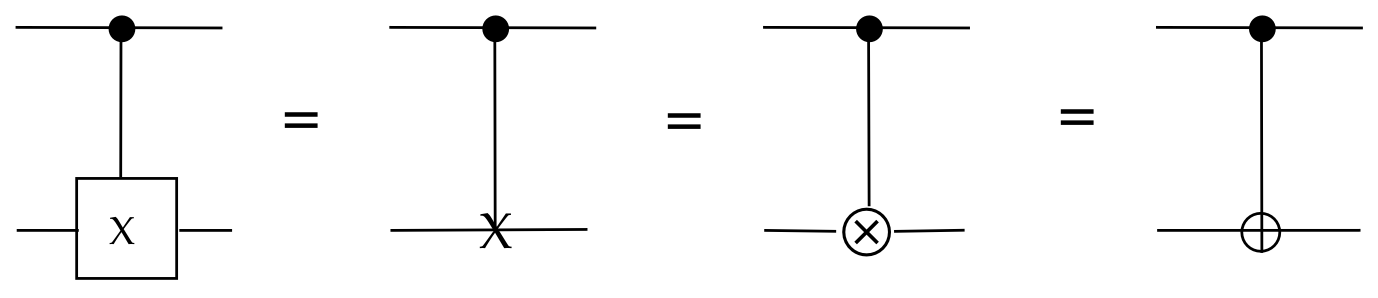
\includegraphics[width=4in]{notes/figs/n08/17cnot.png}
        \caption{circuit-diagram symbols}
        \label{fig:17cnot}
    \end{figure}
    
    In matrix form and Dirac forms:
    
    $$
    C_{N O T}=|0\rangle\langle 0|\otimes I+| 1\rangle\langle 1| \otimes X=\left[\begin{array}{llll}
    1 & 0 & 0 & 0 \\
    0 & 1 & 0 & 0 \\
    0 & 0 & 0 & 1 \\
    0 & 0 & 1 & 0
    \end{array}\right]
    $$
    
    Thus, even though $C_{NOT}$ cannot be written as a direct tensor, it is a sum of two tensors. The top bit is called the control bit when the control bit is either $|0\rangle$ or $|1\rangle$ shown in Figure \ref{fig:18cnot2}.
    
    \begin{figure}
        \centering
        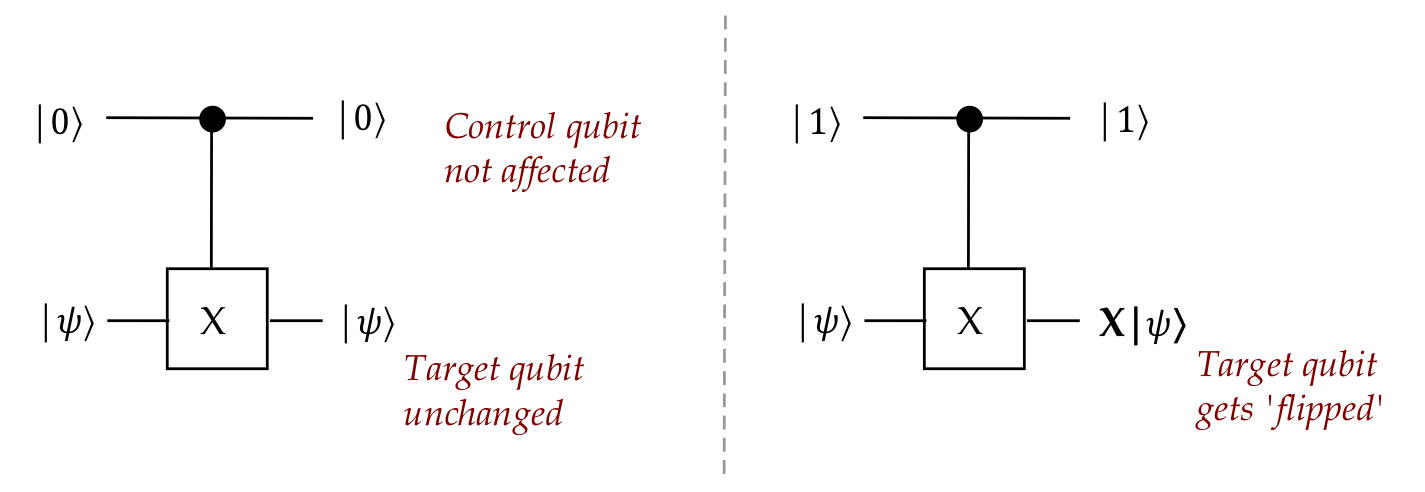
\includegraphics[width=4in]{notes/figs/n08/18cnot2.png}
        \caption{Control Bit}
        \label{fig:18cnot2}
    \end{figure}
    
    $$
    (|0\rangle\langle 0|\otimes I+| 1\rangle\langle 1| \otimes X)(|0\rangle \otimes|\psi\rangle)=|0\rangle \otimes|\psi\rangle
    $$
    
    $$
    (|0\rangle\langle 0|\otimes I+| 1\rangle\langle 1| \otimes X)(|1\rangle \otimes|\psi\rangle)=|1\rangle \otimes X|\psi\rangle
    $$
    
    This 'flipping' does not necessarily happen with other vectors in the control bit:
    
    $$
    \begin{aligned}
    &C_{\text {NOT }}|+,+\rangle=|+,+\rangle \\
    &C_{\text {NOT }}|-,+\rangle=|-,+\rangle
    \end{aligned}
    $$
    
    In neither case does the second change. Summary of properties: $C_{NOT}$ is Hermitian: $C_{NOT}=C_{N O T}^{\dagger}$, $C_{NOT}$ is its own inverse, $C_{NOT}$ can entangle or disentangle.
    
    $$
    \begin{array}{rll}
    \left|\Phi^{+}\right\rangle & =C_{\text {NOT}}|+\rangle|0\rangle & \text { Create entangled Bell state } \\
    C_{N O T}\left|\Phi^{+}\right\rangle & =|+\rangle|0\rangle & C_{NOT} \text { is its own inverse, disentangles Bell state }
    \end{array}
    $$
    
    Important: The term "control" makes sense only when standard-basis vectors are the inputs. We will still use such gates with linear-combinations of standard-basis vectors. In this case, additional reasoning will be needed to ensure the results make sense. $C_{NOT}$ variations: One can easily change the role of the control bit to flip when it's $|0\rangle$ shown in Figure \ref{fig:19cnot3}.
    
    \begin{figure}
        \centering
        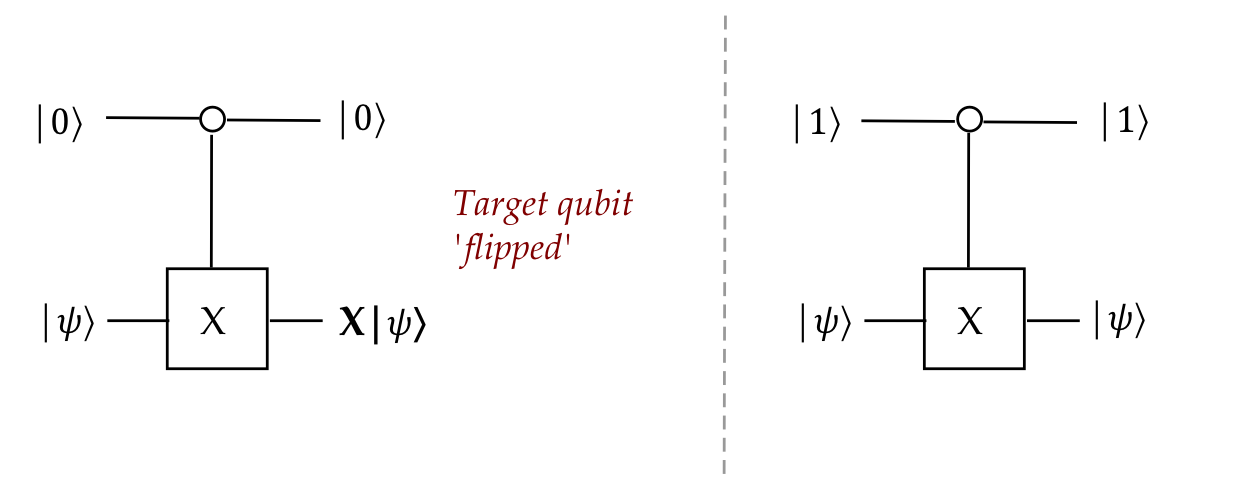
\includegraphics[width=4in]{notes/figs/n08/19cnot3.png}
        \caption{Target qubit flipped}
        \label{fig:19cnot3}
    \end{figure}
    
    $$
    C_{NOT}^{0}=|0\rangle\langle 0|\otimes X+| 1\rangle\langle 1| \otimes I=\left[\begin{array}{llll}
    0 & 1 & 0 & 0 \\
    1 & 0 & 0 & 0 \\
    0 & 0 & 1 & 0 \\
    0 & 0 & 0 & 1
    \end{array}\right]
    $$

    Or make $C_{NOT}$ "upside-down" by using the second qubit as control shown in Figure \ref{fig:20cnot4}.
    
    \begin{figure}
        \centering
        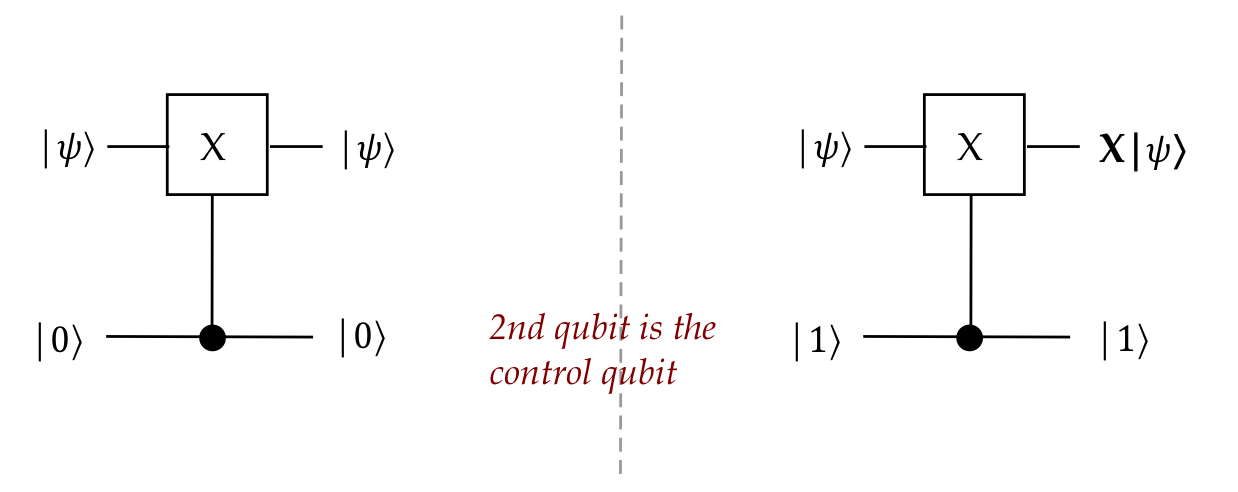
\includegraphics[width=4in]{notes/figs/n08/20cnot4.png}
        \caption{2nd qubit is control bit}
        \label{fig:20cnot4}
    \end{figure}
    
    We'll call this $\bar{C}_{NOT}$. The $C_{Z}$ gate: $C_{Z}=$ Controlled $-Z$. In Dirac and matrix forms:
    
    $$
    C_{Z}=|0\rangle\langle 0|\otimes I+| 1\rangle\langle 1| \otimes Z=\left[\begin{array}{cccc}
    1 & 0 & 0 & 0 \\
    0 & 1 & 0 & 0 \\
    0 & 0 & 1 & 0 \\
    0 & 0 & 0 & -1
    \end{array}\right]
    $$
    
    Similarly, the upside-down version is:
    
    $$
    \bar{C}_{Z}=I \otimes|0\rangle\langle 0|+Z \otimes| 1\rangle\langle 1|
    $$
    
    Surprisingly, $\bar{C}_{Z}=C_{Z}$ referenced in Figure \ref{fig:21cz1}.
    
    \begin{figure}
        \centering
        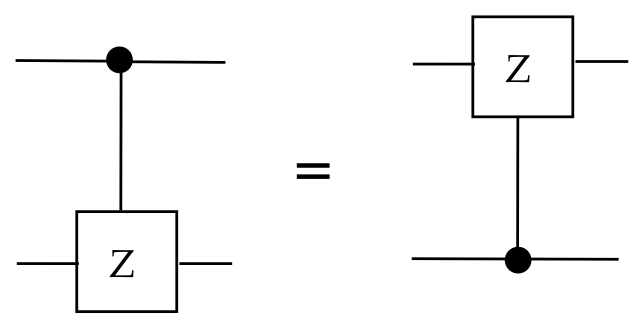
\includegraphics[width=3in]{notes/figs/n08/21cz1.png}
        \caption{$\bar{C}_{Z}=C_{Z}$}
        \label{fig:21cz1}
    \end{figure}
    
    $C_{NOT}$ can be built out of $C_{Z}$ and two 1-qubit Hadamards shown in Figure \ref{fig:22cz2}.
    
    \begin{figure}
        \centering
        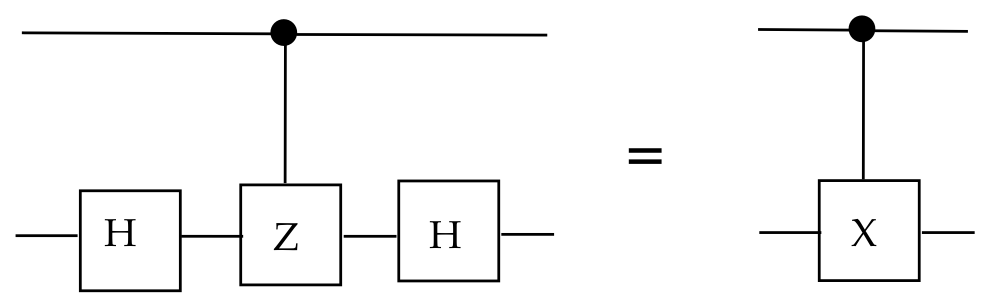
\includegraphics[width=3in]{notes/figs/n08/22cz2.png}
        \caption{$C_{NOT}$ build out}
        \label{fig:22cz2}
    \end{figure}
    
    In some hardware platforms, $C_{Z}$ is easier to implement. Some books use $C_{S I G N}$ as an alternate name for $C_{Z}$. The SWAP gate referenced in Figure \ref{fig:23swap}.
    
    \begin{figure}
        \centering
        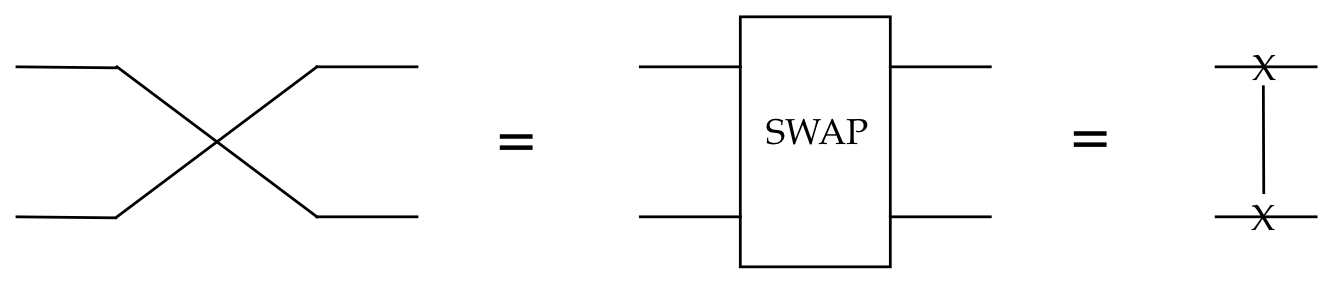
\includegraphics[width=4in]{notes/figs/n08/23swap.png}
        \caption{SWAP}
        \label{fig:23swap}
    \end{figure}
    
    As the name indicates, this gate swaps the states of two qubits. What's important to note: The two qubits themselves don't move. Instead, one's state becomes the other's state. Since there are no "wires" connecting the qubits, it's not obvious this is even feasible. In matrix and Dirac forms:
    
    $$
    \operatorname{SWAP}=|00\rangle\langle 00|+| 01\rangle\langle 10|+| 10\rangle\langle 01|+| 11\rangle\langle 11|=\left[\begin{array}{cccc}
    1 & 0 & 0 & 0 \\
    0 & 0 & 1 & 0 \\
    0 & 1 & 0 & 0 \\
    0 & 0 & 0 & 1
    \end{array}\right]
    $$
    
    Let's first examine what this does to standard-basis qubits shown in Figure \ref{fig:24swap2}.
    
    \begin{figure}
        \centering
        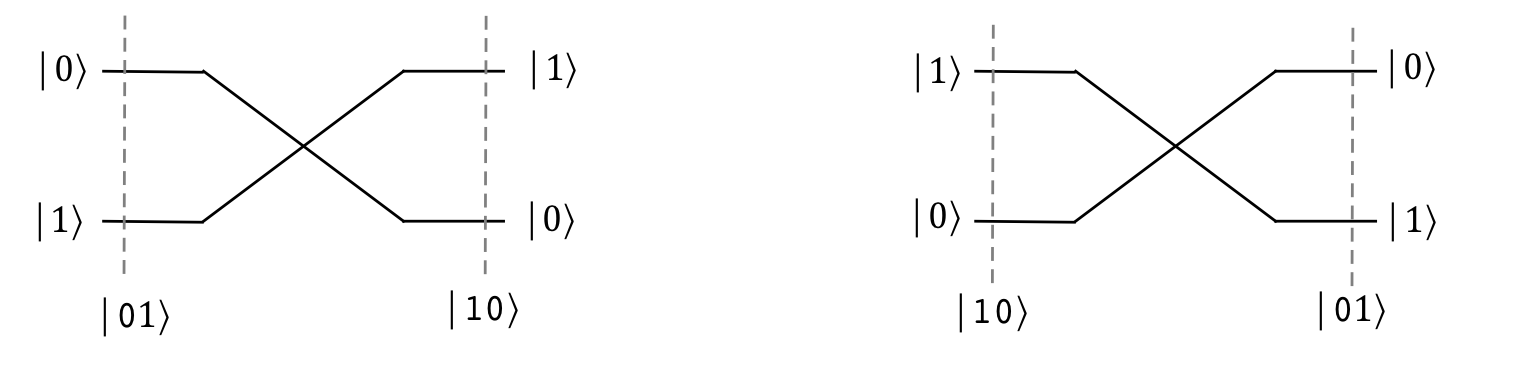
\includegraphics[width=4in]{notes/figs/n08/24swap2.png}
        \caption{standard-basis qubits}
        \label{fig:24swap2}
    \end{figure}

    The Dirac form makes it easy to see what happens with each of these two inputs. When the input is $|01\rangle$ :
    
    $$
    \operatorname{SWAP}|01\rangle=(|00\rangle\langle 00|+| 01\rangle\langle 10|+| 10\rangle\langle 01|+| 11\rangle\langle 11|)|01\rangle=|10\rangle
    $$
    
    For the other case:
    
    $$
    \operatorname{SWAP}|10\rangle=(|00\rangle\langle 00|+| 01\rangle\langle 10|+| 10\rangle\langle 01|+| 11\rangle\langle 11|)|10\rangle=|01\rangle
    $$
    
    We'll now see that arbitrary states get swapped in Figure \ref{fig:25swap3}.
    
    \begin{figure}
        \centering
        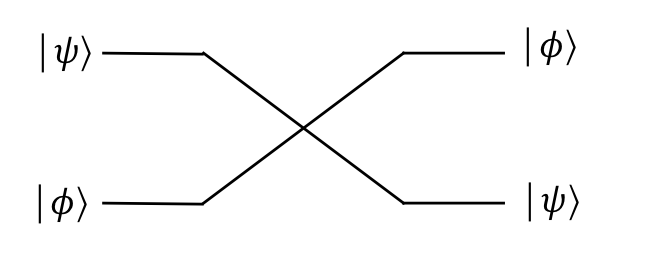
\includegraphics[width=4in]{notes/figs/n08/25swap3.png}
        \caption{arbitrary state swap}
        \label{fig:25swap3}
    \end{figure}
    
    First, via Dirac: Let
    
    $$
    \begin{aligned}
    &|\psi\rangle=\alpha_{1}|0\rangle+\alpha_{2}|1\rangle \\
    &|\phi\rangle=\beta_{1}|0\rangle+\beta_{2}|1\rangle
    \end{aligned}
    $$
    
    Then, applying SWAP to the 2-qubit vector $|\psi\rangle|\phi\rangle$,
    
    $$
    \begin{aligned}
    \operatorname{SWAP}|\psi\rangle|\phi\rangle &=(|00\rangle\langle 00|+| 01\rangle\langle 10|+| 10\rangle\langle 01|+| 11\rangle\langle 11|)\left(\alpha_{1}|0\rangle+\alpha_{2}|1\rangle\right) \otimes\left(\beta_{1}|0\rangle+\beta_{2}|1\rangle\right) \\
    &=(|00\rangle\langle 00|+| 01\rangle\langle 10|+| 10\rangle\langle 01|+| 11\rangle\langle 11|)\left(\alpha_{1} \beta_{1}|00\rangle+\alpha_{1} \beta_{2}|01\rangle \alpha_{2} \beta_{1}|10\rangle+\alpha_{2} \beta_{2}|11\rangle\right) \\
    &=\left(\alpha_{1} \beta_{1}|00\rangle+\alpha_{2} \beta_{1}|01\rangle \alpha_{1} \beta_{2}|10\rangle+\alpha_{2} \beta_{2}|11\rangle\right) \\
    &=\left(\beta_{1} \alpha_{1}|00\rangle+\beta_{1} \alpha_{2}|01\rangle \beta_{2} \alpha_{1}|10\rangle+\beta_{2} \alpha_{2}|11\rangle\right) \\
    &=\left(\beta_{1}|0\rangle+\beta_{2}|1\rangle\right) \otimes\left(\alpha_{1}|0\rangle+\alpha_{2}|1\rangle\right) \\
    &=|\phi\rangle|\psi\rangle
    \end{aligned}
    $$
    
    This is easier to see in matrix form: First, recall how two qubit states are tensored:
    
    $$
    |\psi\rangle|\phi\rangle=\left[\begin{array}{l}
    \alpha_{1} \\
    \alpha_{2}
    \end{array}\right] \otimes\left[\begin{array}{l}
    \beta_{1} \\
    \beta_{2}
    \end{array}\right]=\left[\begin{array}{c}
    \alpha_{1}\left[\begin{array}{l}
    \beta_{1} \\
    \beta_{2}
    \end{array}\right] \\
    \alpha_{2}\left[\begin{array}{l}
    \beta_{1} \\
    \beta_{2}
    \end{array}\right]
    \end{array}\right]=\left[\begin{array}{c}
    \alpha_{1} \beta_{1} \\
    \alpha_{1} \beta_{2} \\
    \alpha_{2} \beta_{1} \\
    \alpha_{2} \beta_{2}
    \end{array}\right]
    $$
    
    Now apply SWAP:
    
    $$
    \begin{aligned}
    &\operatorname{SWAP}|\psi\rangle|\phi\rangle=\left[\begin{array}{cccc}
    1 & 0 & 0 & 0 \\
    0 & 0 & 1 & 0 \\
    0 & 1 & 0 & 0 \\
    0 & 0 & 0 & 1
    \end{array}\right]\left[\begin{array}{l}
    \alpha_{1} \beta_{1} \\
    \alpha_{1} \beta_{2} \\
    \alpha_{2} \beta_{1} \\
    \alpha_{2} \beta_{2}
    \end{array}\right]\\
    &=\left[\begin{array}{c}
    \alpha_{1} \beta_{1} \\
    \alpha_{2} \beta_{1} \\
    \alpha_{1} \beta_{2} \\
    \alpha_{2} \beta_{2}
    \end{array}\right]\\
    &=\left[\begin{array}{l}
    \beta_{1} \alpha_{1} \\
    \beta_{1} \alpha_{2} \\
    \beta_{2} \alpha_{1} \\
    \beta_{2} \alpha_{2}
    \end{array}\right]\\
    &=\left[\begin{array}{l}
    \beta_{1}\left[\begin{array}{l}
    \alpha_{1} \\
    \alpha_{2}
    \end{array}\right] \\
    \beta_{2}\left[\begin{array}{l}
    \alpha_{1} \\
    \alpha_{2}
    \end{array}\right]
    \end{array}\right]\\
    &=|\phi\rangle|\psi\rangle
    \end{aligned}
    $$
    
    SWAP is Hermitian and its own inverse. (It is of course unitary, otherwise it would not be a valid gate.) Fractional powers can be calculated in the usual way to get:
    
    $$
    \sqrt{\text { SWAP }}=\frac{1}{2}\left[\begin{array}{cccc}
    2 & 0 & 0 & 0 \\
    0 & 1+i & 1-1 & 0 \\
    0 & 1-i & 1+i & 0 \\
    0 & 0 & 0 & 2
    \end{array}\right]
    $$
    
    There are other variations of SWAP that are easier to implement on some hardware platforms. Some of these can be combined to create $C_{NOT}$. And three $C_{NOT}$'s can be combined to create SWAP shown in Figure \ref{fig:26swap4}.
    
    \begin{figure}
        \centering
        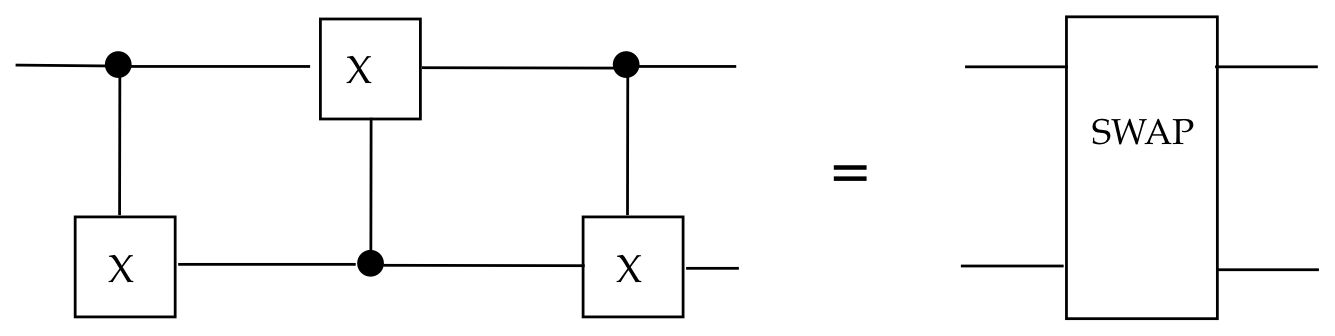
\includegraphics[width=4in]{notes/figs/n08/26swap4.png}
        \caption{arbitrary state swap}
        \label{fig:26swap4}
    \end{figure}
    
    $$
    \text{SWAP}=C_{NOT} \bar{C}_{N O T} C_{N O T}
    $$

    Multiple SWAPs can be used to achieve two-qubit swapping amongst $n$ qubits shown in Figure \ref{fig:27swap5}.
    
    \begin{figure}
        \centering
        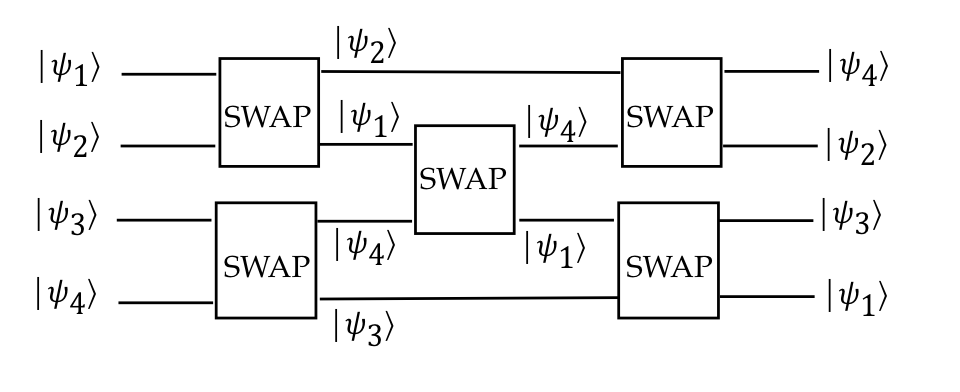
\includegraphics[width=4in]{notes/figs/n08/27swap5.png}
        \caption{two-qubit swapping}
        \label{fig:27swap5}
    \end{figure}
    
    The first and fourth qubit states get swapped through a series of mirrored swaps.
    
\subsection{Multiply-controlled gates}

    The overall goal: Apply a gate to the k-th qubit only when other qubits are in a certain state. Let's first examine one of the most important such gates: $CC_{NOT}$ shown in Figure \ref{fig:28ccnot}.
    
    \begin{figure}
        \centering
        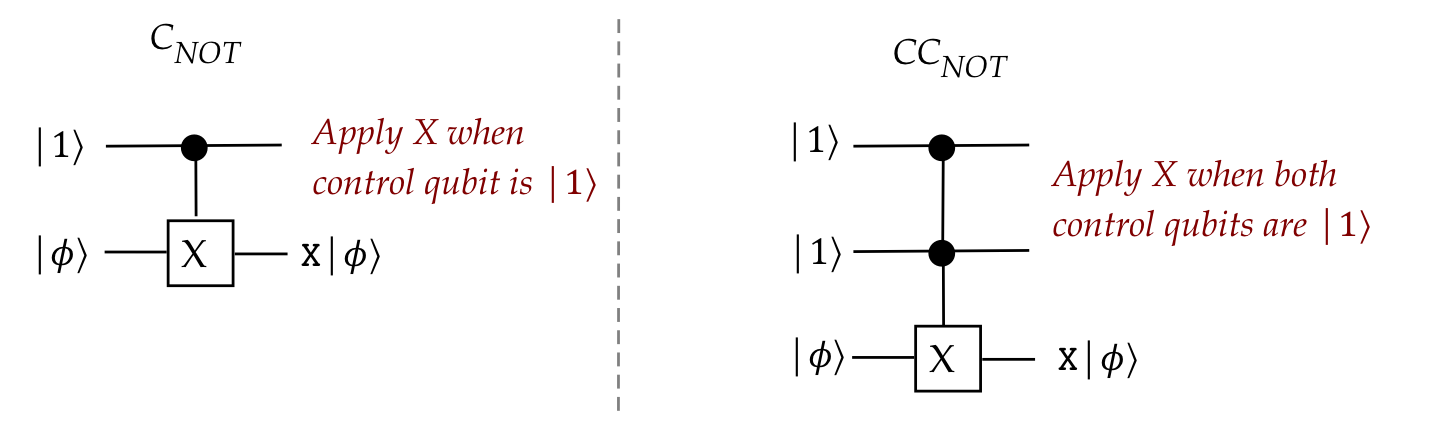
\includegraphics[width=4in]{notes/figs/n08/28ccnot.png}
        \caption{two-qubit swapping}
        \label{fig:28ccnot}
    \end{figure}
    
    Suppose we want a 3-qubit gate where the first two qubits "control" the third, as shown on the right. In this case, what we seek is: When the first two qubits both have state $|1\rangle$, then "flip" (apply $X$ ) to the third. In all other cases, leave the third qubit as is. And: the control qubits are unchanged. We can write this as:
    
    $$
    \begin{aligned}
    C C_{\text {NOT }}|\psi\rangle &=|\psi\rangle \quad|\psi\rangle \in(|000\rangle,|001\rangle,|010\rangle,|011\rangle,|100\rangle,|101\rangle) \\
    C C_{\text {NOT }}|110\rangle &=|111\rangle \\
    C C_{\text {NOT }}|111\rangle &=|110\rangle
    \end{aligned}
    $$
    
    Thus,
    
    $$
    \begin{aligned}
    &C C_{\text {NOT }} \\
    &=|000\rangle\langle 000|+\ldots+| 101\rangle\langle\mathbf{1 0 1}|+| \mathbf{1 1 0}\rangle\langle\mathbf{1 1 1}|+| \mathbf{1 1 1}\rangle\langle\mathbf{1 1 0}| \\
    &=\left[\begin{array}{llllllll}
    1 & 0 & 0 & 0 & 0 & 0 & 0 & 0 \\
    0 & 1 & 0 & 0 & 0 & 0 & 0 & 0 \\
    0 & 0 & 1 & 0 & 0 & 0 & 0 & 0 \\
    0 & 0 & 0 & 1 & 0 & 0 & 0 & 0 \\
    0 & 0 & 0 & 0 & 1 & 0 & 0 & 0 \\
    0 & 0 & 0 & 0 & 0 & 1 & 0 & 0 \\
    0 & 0 & 0 & 0 & 0 & 0 & 0 & \mathbf{1} \\
    0 & 0 & 0 & 0 & 0 & 0 & \mathbf{1} & 0
    \end{array}\right]
    \end{aligned}
    $$
    
    Of course, just because we make up a unitary operation doesn't necessarily mean it's easy to implement in real hardware. $\triangleright$ We'll address this issue in a later section in this module. Once we have such a gate, one can use additional gates to specify other types of control: For example, suppose we want to apply $X$ to the third qubit when the first two are in state $|10\rangle$. In this case one can add an $X$ before the 2nd qubit shown in Figure \ref{fig:29ccnot2}.
    
    \begin{figure}
        \centering
        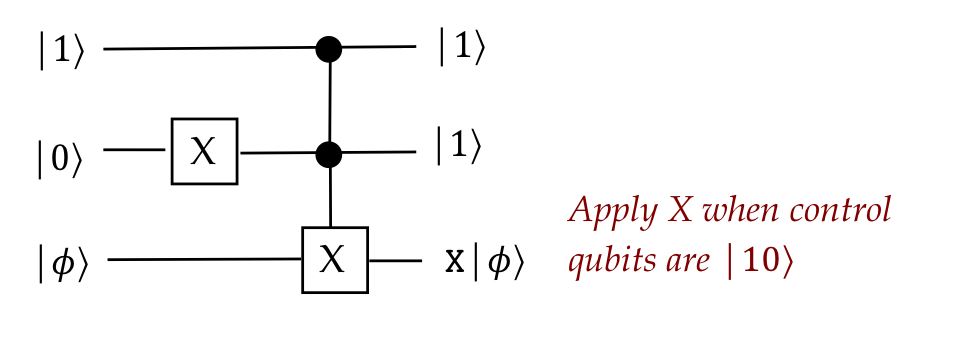
\includegraphics[width=4in]{notes/figs/n08/29ccnot2.png}
        \caption{Apply X}
        \label{fig:29ccnot2}
    \end{figure}
    
    Notice that the second control bit was modified. To restore, one can "undo" the $X$ on the second bit shown in Figure \ref{fig:30ccnot3}.
    
    \begin{figure}
        \centering
        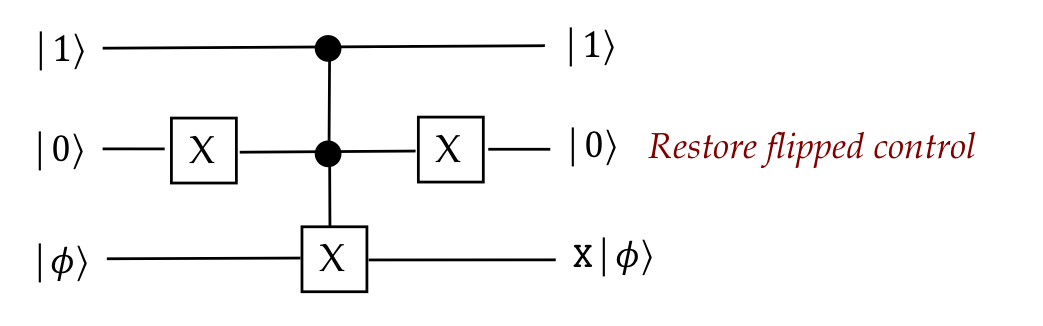
\includegraphics[width=4in]{notes/figs/n08/30ccnot3.png}
        \caption{Restore}
        \label{fig:30ccnot3}
    \end{figure}
    
    Note: The "control" has been set up for standard basis vectors. However, the third qubit can be in any state. Of course, nothing prevents us from applying the circuit to arbitrary vectors, if that's useful. Terminology: $CC_{NOT}=$ Controlled-controlled-NOT

\subsection{Common 3-qubit gates}

    We've already seen the first important 3-qubit gate, $C C_{N O T}$, also known as the Toffoli gate shown in Figure \ref{fig:30ccnot3}.
    
    \begin{figure}
        \centering
        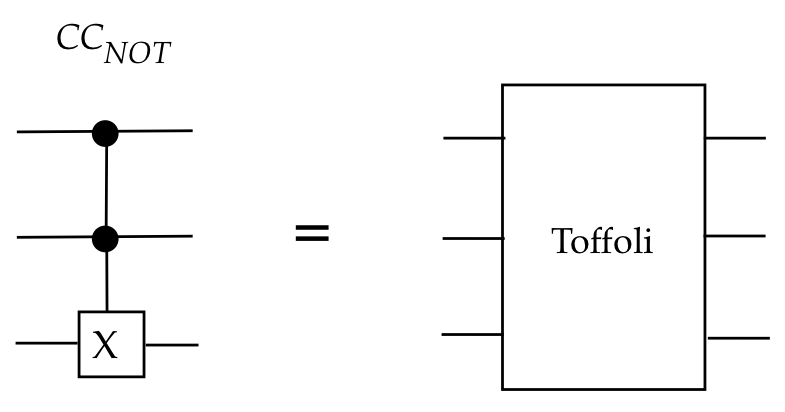
\includegraphics[width=4in]{notes/figs/n08/31toffoli.png}
        \caption{Toffoli}
        \label{fig:31toffoli}
    \end{figure}
    
    Three qubit gates such as the Toffoli and Fredkin (below), are valuable because they can be used for many purposes. However, a 3-qubit gate is difficult to implement in practice because it involves a physical action on three qubits, even if swapping brings them in the same vicinity. The Toffoli gate can be implemented using ten 1-qubit gates and six $C_{NOT} \mathrm{~s}$ shown in Figure \ref{fig:32toffoli2}.
    
    \begin{figure}
        \centering
        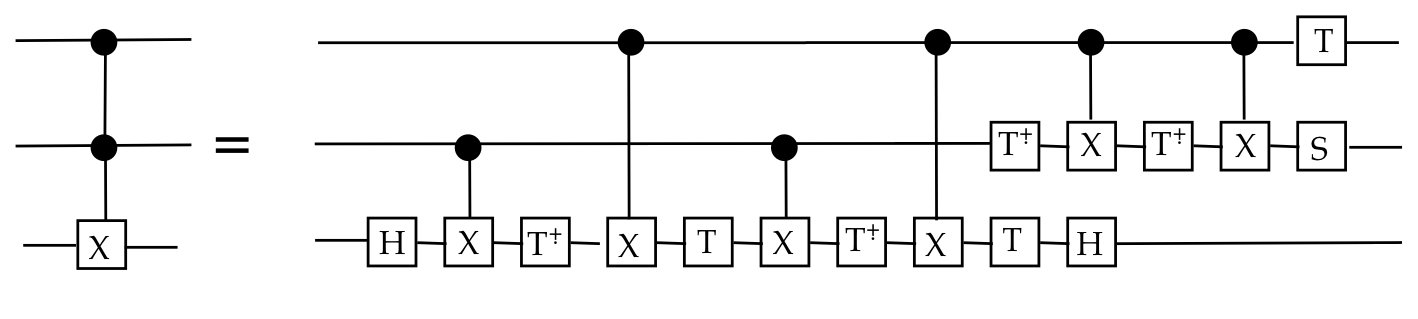
\includegraphics[width=4in]{notes/figs/n08/32toffoli2.png}
        \caption{Toffoli ten 1-qubit}
        \label{fig:32toffoli2}
    \end{figure}
    
    Recall:
    
    $$
    \begin{aligned}
    S &=\left[\begin{array}{ll}
    1 & 0 \\
    0 & i
    \end{array}\right] \\
    T &=\left[\begin{array}{cc}
    1 & 0 \\
    0 & e^{i \frac{\pi}{4}}
    \end{array}\right] \\
    T^{\dagger} &=\left[\begin{array}{cc}
    1 & 0 \\
    0 & e^{-i \frac{\pi}{4}}
    \end{array}\right]
    \end{aligned}
    $$
    
    Instead of working through the details, we'll highlight a few points shown in Figure \ref{}.
    
    \begin{figure}
        \centering
        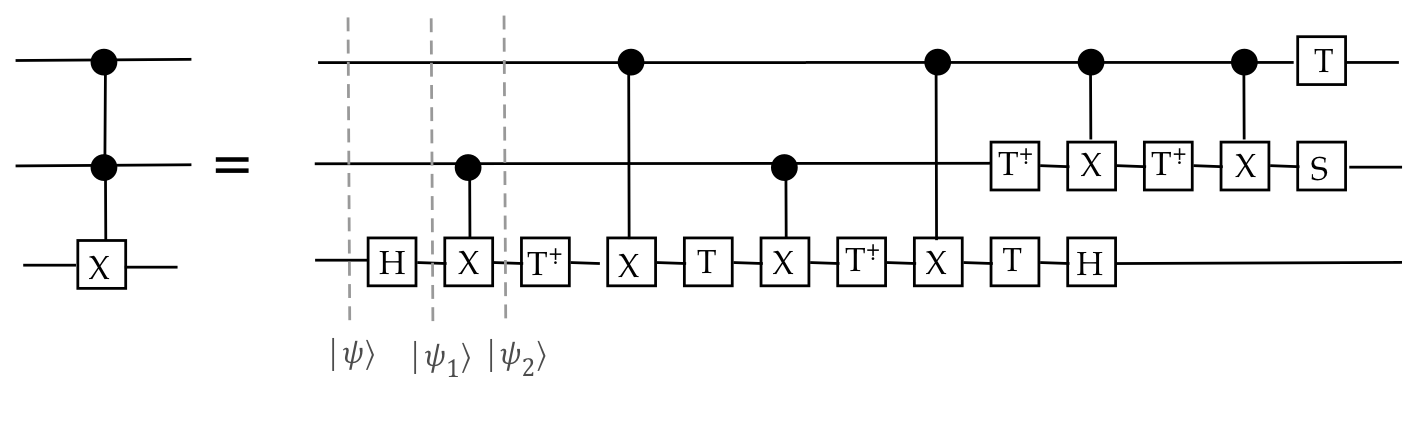
\includegraphics[width=4in]{notes/figs/n08/33toffoli3.png}
        \caption{$|\psi\rangle$ progression}
        \label{fig:33toffoli3}
    \end{figure}
    
    Suppose the input is $|\psi\rangle$. The first 3-qubit unitary comes from producing $\left|\psi_{1}\right\rangle$ :
    
    $$
    \left|\psi_{1}\right\rangle=(I \otimes I \otimes H)|\psi\rangle
    $$
    
    The next one is:
    
    $$
    \left|\psi_{2}\right\rangle=\left(I \otimes C_{N O T}\right)\left|\psi_{1}\right\rangle=\left(I \otimes C_{N O T}\right)(I \otimes I \otimes H)|\psi\rangle
    $$
    
    And so on. Notice the $C_{NOT}$ between the first and third qubits. If these aren't physically adjacent it may be difficult to get $C_{NOT}$ to work. There are alternative circuits that use only adjacent-qubit $C_{N O T} \mathrm{~s}$ (8 of them). The above complicated breakdown into $C_{NOT}$ gates is difficult to understand, and came about through clever trial and error. Let's look at a more understandable decomposition using $C_{NOT}$ gates and $\sqrt{X}$ shown in Figure \ref{fig:34ccnot4}.
    
    \begin{figure}
        \centering
        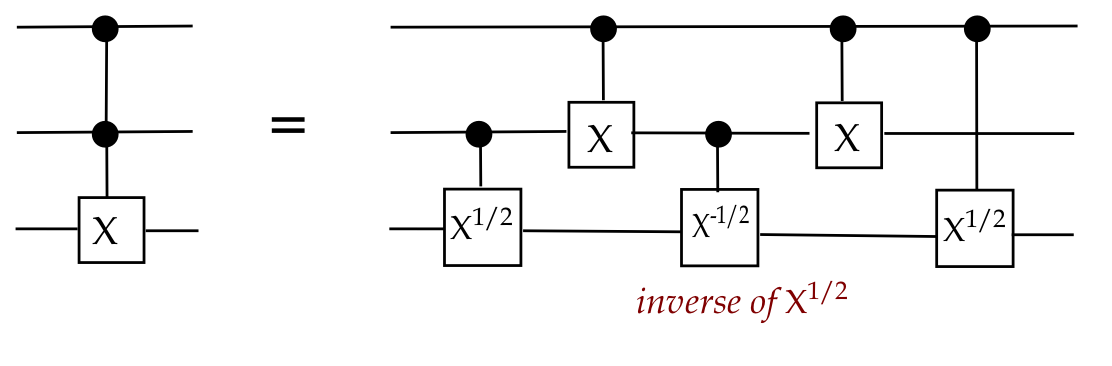
\includegraphics[width=4in]{notes/figs/n08/34ccnot4.png}
        \caption{Decomposition using $C_{NOT}$ gates and $\sqrt{X}$}
        \label{fig:34ccnot4}
    \end{figure}
    
    Just as Controlled- $X$ is a gate, suppose we could build Controlled $-\sqrt{X}$ and its inverse Controlled $X^{-\frac{1}{2}}$. Construction of a generic Controlled- $U$ is shown in a section below. Now consider the different control-qubit combinations $|0\rangle|0\rangle,|0\rangle|1\rangle,|1\rangle|0\rangle,|1\rangle|1\rangle$. With $|0\rangle|0\rangle$, none of the controls are activated, so the third qubit merely passes through shown in Figure \ref{fig:35ccnot5}.
    
    \begin{figure}
        \centering
        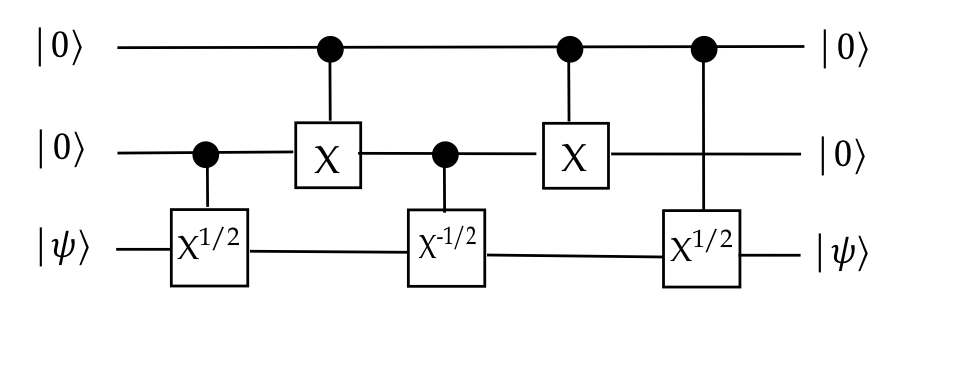
\includegraphics[width=4in]{notes/figs/n08/35ccnot5.png}
        \caption{third qubit pass through}
        \label{fig:35ccnot5}
    \end{figure}

    With $|0\rangle|1\rangle$, the two highlighted gates are activated but cancel out (the second is the inverse of the first) shown in Figure \ref{fig:36ccnot6}.
    
    \begin{figure}
        \centering
        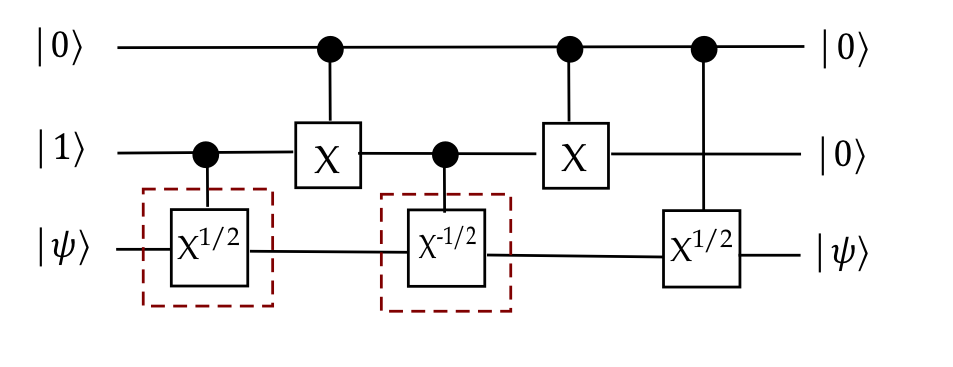
\includegraphics[width=4in]{notes/figs/n08/36ccnot6.png}
        \caption{$|0\rangle|1\rangle$ activated gates}
        \label{fig:36ccnot6}
    \end{figure}
    
    With $|1\rangle|0\rangle$ shown in Figure \ref{fig:37ccnot7}.
    
    \begin{figure}
        \centering
        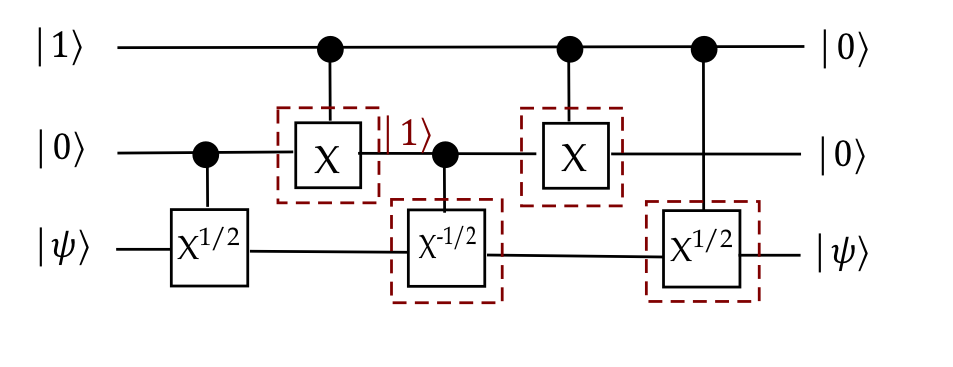
\includegraphics[width=4in]{notes/figs/n08/37ccnot7.png}
        \caption{$|1\rangle|0\rangle$ activated gates}
        \label{fig:37ccnot7}
    \end{figure}
    
    And finally, $|1\rangle|1\rangle$ results in the two $\sqrt{X}$ gates multiplying to produce the desired $X$ on the third qubit shown in Figure \ref{fig:38ccnot8}.
    
    \begin{figure}
        \centering
        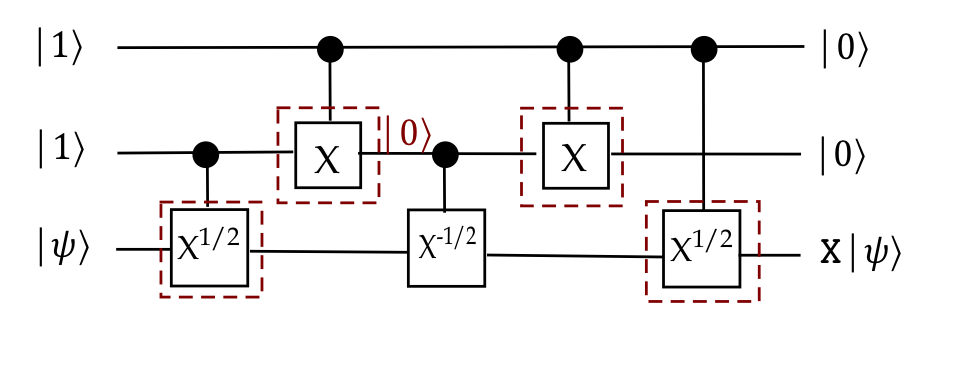
\includegraphics[width=4in]{notes/figs/n08/38ccnot8.png}
        \caption{$|1\rangle|1\rangle$ activated gates}
        \label{fig:38ccnot8}
    \end{figure}
    
    The Toffoli gate is its own inverse, which is easy to see graphically in Figure \ref{fig:39toffoli4}.
    
    \begin{figure}
        \centering
        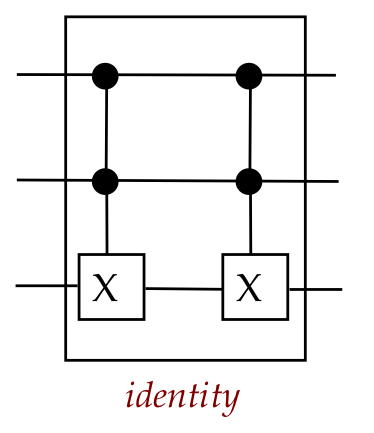
\includegraphics[width=2in]{notes/figs/n08/39toffoli4.png}
        \caption{Toffoli gate is its own inverse}
        \label{fig:39toffoli4}
    \end{figure}
    
    The Toffoli gate is named in honor of Tommasso Toffoli, who first proposed the gate (in a classical context). 
    
    The Fredkin gate is shown in Figure \ref{fig:40fredkin}.
    
    \begin{figure}
        \centering
        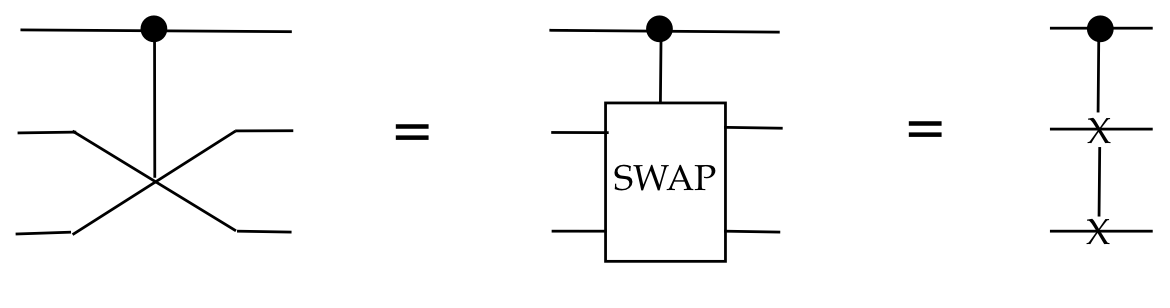
\includegraphics[width=4in]{notes/figs/n08/40fredkin.png}
        \caption{Fredkin}
        \label{fig:40fredkin}
    \end{figure}
    
    Also called Controlled-SWAP. The idea is to use the first bit (in standard-basis) to decide whether to swap the other two:
    
    $$
    \begin{aligned}
    \text { C-SWAP }|\psi\rangle &=|\psi\rangle \quad|\psi\rangle \in(|000\rangle,|001\rangle,|010\rangle,|011\rangle,|100\rangle,|111\rangle) \\
    \text { C-SWAP }|101\rangle &=|110\rangle \\
    \text { C-SWAP }|110\rangle &=|101\rangle
    \end{aligned}
    $$
    
    In Dirac and matrix form:
    
    $$
    \begin{aligned}
    &\text { C-SWAP } \\
    &=|000\rangle\langle 000|+\ldots+| 100\rangle\langle 100|+| 111\rangle+|\mathbf{1 0 1}\rangle \\
    &=\left[\begin{array}{llllllll}
    1 & 0 & 0 & 0 & 0 & 0 & 0 & 0 \\
    0 & 1 & 0 & 0 & 0 & 0 & 0 & 0 \\
    0 & 0 & 1 & 0 & 0 & 0 & 0 & 0 \\
    0 & 0 & 0 & 1 & 0 & 0 & 0 & 0 \\
    0 & 0 & 0 & 0 & 1 & 0 & 0 & 0 \\
    0 & 0 & 0 & 0 & 0 & 0 & \mathbf{1} & 0 \\
    0 & 0 & 0 & 0 & 0 & \mathbf{1} & 0 & 0 \\
    0 & 0 & 0 & 0 & 0 & 0 & 0 & 1
    \end{array}\right]
    \end{aligned}
    $$
    
    One can see the structure in the matrix:
    
    $$
    \mathrm{C}-\mathrm{SWAP}=|0\rangle\langle 0|\otimes I \otimes I+| 1\rangle\langle 1| \otimes \mathrm{SWAP}
    $$
    
    Let's confirm that it does work as intended when the 2nd and 3rd qubits are in generic states: Let
    
    $$
    \begin{aligned}
    &\left|\phi_{1}\right\rangle=\alpha_{1}|0\rangle+\beta_{1}|1\rangle \\
    &\left|\phi_{2}\right\rangle=\alpha_{2}|0\rangle+\beta_{2}|1\rangle
    \end{aligned}
    $$
    
    be the 2nd and 3rd qubits. Next, let's compute the two cases (first qubit $|0\rangle$ vs. $|1\rangle$ )

    $$
    \begin{aligned}
    |0\rangle\left|\phi_{1}\right\rangle\left|\phi_{2}\right\rangle &=|0\rangle\left(\alpha_{1}|0\rangle+\beta_{1}|1\rangle\right)\left(\alpha_{2}|0\rangle+\beta_{2}|1\rangle\right) \\
    &=\alpha_{1} \alpha_{2}|000\rangle+\alpha_{1} \beta_{2}|001\rangle+\beta_{1} \alpha_{2}|010\rangle+\beta_{1} \beta_{2}|011\rangle
    \end{aligned}
    $$
    
    The other:
    
    $$
    \begin{aligned}
    |1\rangle\left|\phi_{1}\right\rangle\left|\phi_{2}\right\rangle &=|1\rangle\left(\alpha_{1}|0\rangle+\beta_{1}|1\rangle\right)\left(\alpha_{2}|0\rangle+\beta_{2}|1\rangle\right) \\
    &=\alpha_{1} \alpha_{2}|100\rangle+\alpha_{1} \beta_{2}|101\rangle+\beta_{1} \alpha_{2}|110\rangle+\beta_{1} \beta_{2}|111\rangle
    \end{aligned}
    $$
    
    Then when the first qubit is $|0\rangle$. C-SWAP $|0\rangle\left|\phi_{1}\right\rangle\left|\phi_{2}\right\rangle$
    
    $$
    \begin{aligned}
    &=(|000\rangle\langle 000|+\ldots+| 100\rangle\langle 100|+| 111\rangle\langle 111|+| 101\rangle\langle\mathbf{1 1 0}|+| 110\rangle\langle\mathbf{1 0 1}|)|0\rangle\left|\phi_{1}\right\rangle\left|\phi_{1}\right\rangle \\
    &=\alpha_{1} \alpha_{2}|000\rangle+\alpha_{1} \beta_{2}|001\rangle+\beta_{1} \alpha_{2}|010\rangle+\beta_{1} \beta_{2}|011\rangle \\
    &=|0\rangle\left|\phi_{1}\right\rangle\left|\phi_{2}\right\rangle
    \end{aligned}
    $$
    
    Thus, unchanged, as required. Note: neither of the two bolded outer-products match against any vector in the expansion of $|0\rangle\left|\phi_{1}\right\rangle\left|\phi_{2}\right\rangle$.
    
    On the other hand,
    
    $$
    \begin{aligned}
    & \text { C-SWAP }|1\rangle\left|\phi_{1}\right\rangle\left|\phi_{2}\right\rangle \\
    =&(|000\rangle\langle 000|+\ldots+| 100\rangle\langle 100|+| 111\rangle\langle 111|+| 101\rangle\langle\mathbf{1 1 0}|+| 110\rangle\langle\mathbf{1 0 1}|)|0\rangle\left|\phi_{1}\right\rangle\left|\phi_{1}\right\rangle \\
    =&(|000\rangle\langle 000|+\ldots+| 100\rangle\langle 100|+| 111\rangle+|101\rangle\langle\mathbf{1 1 0}|+| 110\rangle\langle\mathbf{1 0 1}|) \\
    &\left(\alpha_{1} \alpha_{2}|100\rangle+\alpha_{1} \beta_{2}|\mathbf{1 0 1}\rangle+\beta_{1} \alpha_{2}|\mathbf{1 1 0}\rangle+\beta_{1} \beta_{2}|111\rangle\right) \\
    =& \alpha_{1} \alpha_{2}|100\rangle+\alpha_{1} \beta_{2}|110\rangle+\beta_{1} \alpha_{2}|101\rangle+\beta_{1} \beta_{2}|111\rangle \\
    =&|1\rangle \otimes\left(\alpha_{2}|0\rangle+\beta_{2}|1\rangle\right)\left(\alpha_{1}|0\rangle+\beta_{1}|1\rangle\right) \\
    =&|1\rangle\left|\phi_{2}\right\rangle\left|\phi_{1}\right\rangle
    \end{aligned}
    $$
    
    As desired. CSWAP can be implemented with two $C_{NOT}$ gates and one $CC_{NOT}$ shown in Figure \ref{fig:41fredkin2}.
    
    \begin{figure}
        \centering
        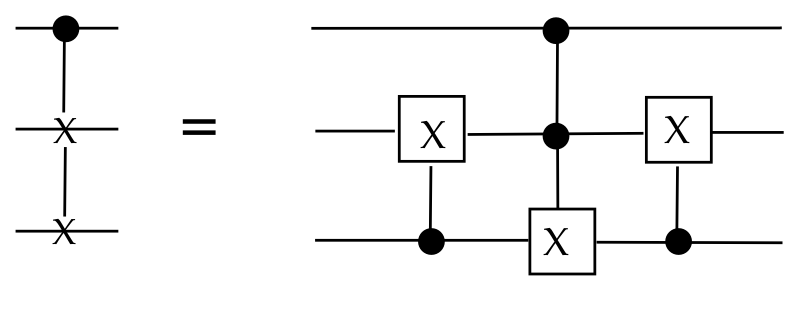
\includegraphics[width=4in]{notes/figs/n08/41fredkin2.png}
        \caption{CSWAP}
        \label{fig:41fredkin2}
    \end{figure}
    
    Let's work out a few steps: The product of the three stages is:
    
    $$
    \left(I \otimes \bar{C}_{N O T}\right) C C_{N O T}\left(I \otimes \bar{C}_{N O T}\right)
    $$
    
    The first term is:
    
    $$
    \begin{aligned}
    I \otimes \bar{C}_{\text {NOT }}=& I \otimes(I \otimes|0\rangle\langle 0|+X \otimes| 1\rangle\langle 1|) \\
    =& I \otimes I \otimes|0\rangle\langle 0|+I \otimes X \otimes| 1\rangle\langle 1| \\
    =&(|00\rangle\langle 00|+| 01\rangle\langle 01|+| 10\rangle\langle 10|+| 11\rangle\langle 11|) \otimes|0\rangle\langle 0| \\
    &+(|00\rangle\langle 01|+| 01\rangle\langle 00|+| 10\rangle\langle 11|+| 11\rangle\langle 10|) \otimes|1\rangle\langle 1| \\
    =&|000\rangle\langle 000|+| 010\rangle\langle 010|+| 100\rangle\langle 100|+| 110\rangle\langle 110| \\
    &|001\rangle\langle 011|+| 011\rangle\langle 001|+| 101\rangle\langle 111|+| 111\rangle\langle 101|
    \end{aligned}
    $$
    
    This gate is named in honor of Ed Fredkin, who proposed the gate, and who had an interesting career. The $CC_{Z}$ gate is shown in Figure \ref{fig:42ccz}.
    
    \begin{figure}
        \centering
        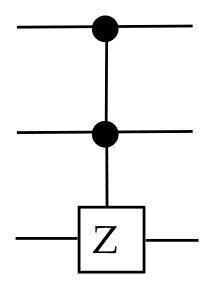
\includegraphics[width=4in]{notes/figs/n08/42ccz.png}
        \caption{$CC_{Z}$ gate}
        \label{fig:42ccz}
    \end{figure}
    
    As the name implies, if the first two qubits are in state $|1\rangle$ then $Z$ is applied to the third qubit. In Dirac and matrix form:
    
    $$
    \begin{aligned}
    &C C_{Z} \\
    &= \\
    &=\left[\begin{array}{lllllllc}
    1 & 0 & 0 & 0 & 0 & 0 & 0 & 0 \\
    0 & 1 & 0 & 0 & 0 & 0 & 0 & 0 \\
    0 & 0 & 1 & 0 & 0 & 0 & 0 & 0 \\
    0 & 0 & 0 & 1 & 0 & 0 & 0 & 0 \\
    0 & 0 & 0 & 0 & 1 & 0 & 0 & 0 \\
    0 & 0 & 0 & 0 & 0 & 1 & 0 & 0 \\
    0 & 0 & 0 & 0 & 0 & 0 & 1 & 0 \\
    0 & 0 & 0 & 0 & 0 & 0 & 0 & -\mathbf{1}
    \end{array}\right]
    \end{aligned}
    $$
    
    Just as $C_{Z}$ can be implemented with $C_{NOT}$, so can $CC_{Z}$ shown in Figure \ref{fig:42ccz}.
    
    \begin{figure}
        \centering
        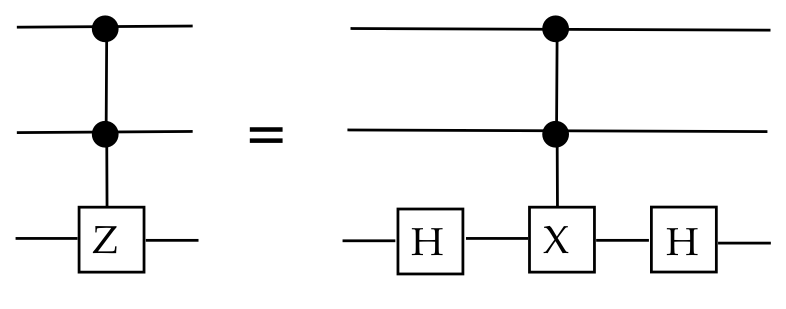
\includegraphics[width=4in]{notes/figs/n08/43ccz2.png}
        \caption{$CC_{Z}$ implemented with $C_{NOT}$}
        \label{fig:43ccz2}
    \end{figure}
    
    That is,
    
    $$
    C C_{Z}=(I \otimes I \otimes H) C C_{NOT}(I \otimes I \otimes H)
    $$
    
\subsection{A useful trick: control vector conversion}

    In some applications, it's useful to be able to transform an output vector so that controls can be applied in a certain pre-configured way. For example, in a 3-qubit case, suppose the input is known to $|001\rangle$ and we want to convert this to $|000\rangle$ shown in Figure \ref{fig:44convert}.
    
    \begin{figure}
        \centering
        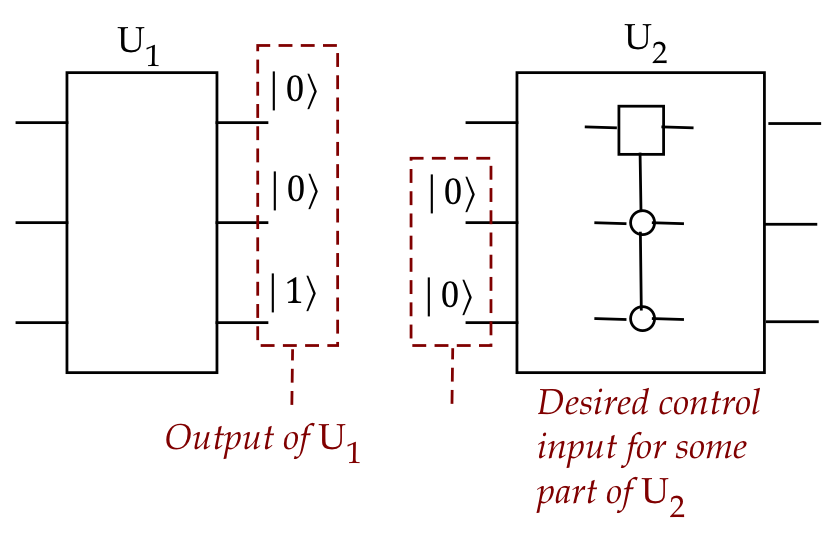
\includegraphics[width=4in]{notes/figs/n08/44convert.png}
        \caption{Transform output vector}
        \label{fig:44convert}
    \end{figure}
    
    In this case, the $|001\rangle$ is the output of some circuit $U_{1}$. The circuit $U_{2}$ needs the latter 2 bits of the input to be $|x 00\rangle$, where $x$ is either 0 or 1 . This can be achieved through a $C_{NOT}$ shown in Figure \ref{fig:45convert2}.
    
    \begin{figure}
        \centering
        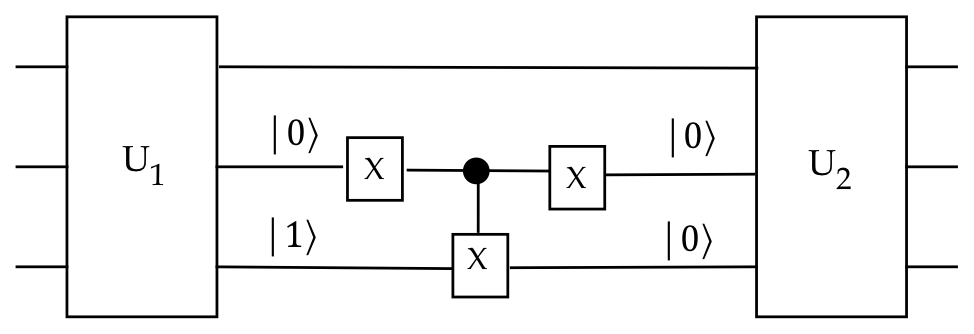
\includegraphics[width=4in]{notes/figs/n08/45convert2.png}
        \caption{Output vector transform achieved through $C_{NOT}$}
        \label{fig:45convert2}
    \end{figure}
    
    Note: the control state is $|0\rangle$. Why don't we simply apply $X$ to the 3rd qubit? Our goal is to have this transformation apply only when the input is $|x 01\rangle$ (latter two in state $|01\rangle$. Then, other inputs will not be affected. Next, suppose we wish to convert $|x 01\rangle$ to $|x 10\rangle$. In this case, a single bit-flip amongst the 2nd and 3rd qubits is not sufficient. We can instead use two $C_{\text {Not}}$ gates. To do this, we first flip one state bit (3rd qubit) going from $|x 01\rangle \rightarrow|x 00\rangle$. And then $|x 00\rangle \rightarrow|x 10\rangle$ as shown in Figure \ref{fig:46convert4}.
    
    \begin{figure}
        \centering
        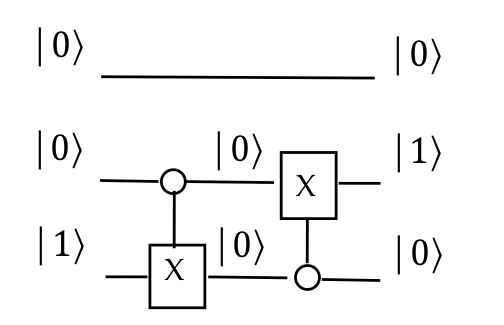
\includegraphics[width=4in]{notes/figs/n08/46convert4.png}
        \caption{convert $|x 01\rangle$ to $|x 10\rangle$}
        \label{fig:46convert4}
    \end{figure}
    
    Notice that our drawing now reflects the use of $|0\rangle$ as control (open circle in the drawing). In general, several steps may be needed to flip one bit at a time to transition from one set of input qubits to another with desired controls. For example, suppose one wants to convert $|100 x\rangle$ to $|011 x\rangle$. Then, the following steps would work:
    
    $$
    |100 x\rangle \rightarrow|000 x\rangle \rightarrow|010 x\rangle \rightarrow|011 x\rangle
    $$

    Each step is a controlled-flip, controlled by the other three bits.

\subsection{Caveats}

    First, as we've seen before, the notion of "control" can be ambiguous: Recall the difference between standard-basis and Hadamard for $C_{NOT}$ shown in Figure \ref{fig:47caveat1}.
    
    \begin{figure}
        \centering
        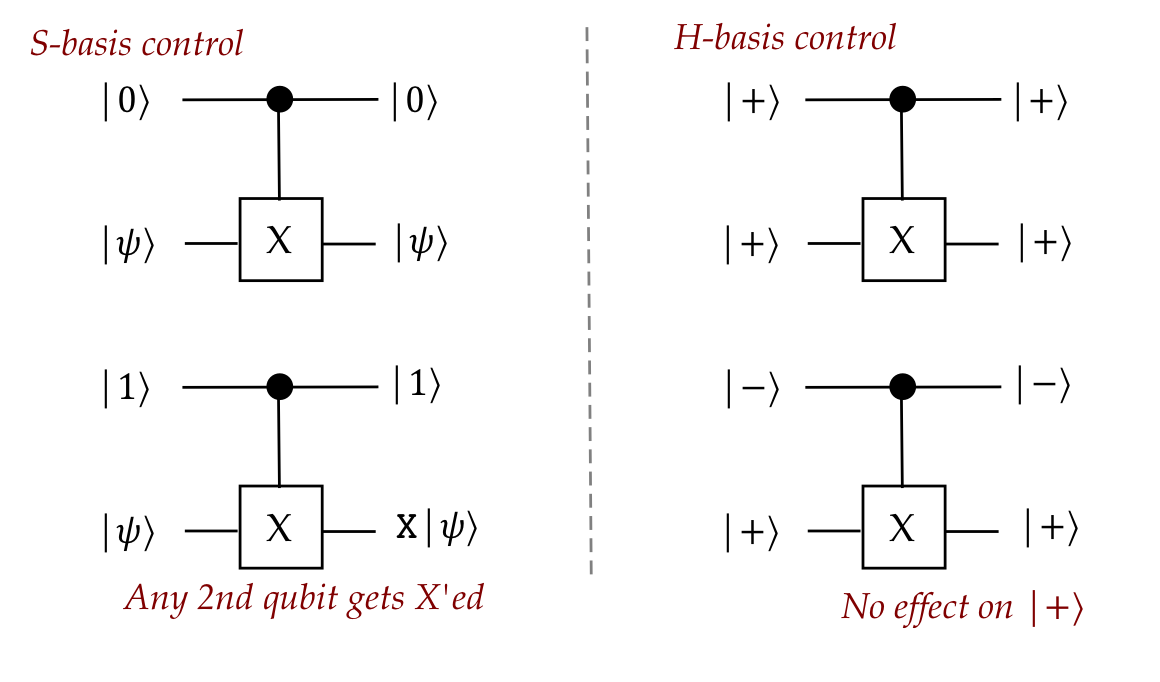
\includegraphics[width=4in]{notes/figs/n08/47caveat1.png}
        \caption{Difference between standard-basis and Hadamard}
        \label{fig:47caveat1}
    \end{figure}
    
    With standard-basis control qubits, we get the desired behavor, when the control-qubit is $|0\rangle$, there is no change to the second. When it's $|1\rangle, X$ gets applied to any second qubit state.
    Instead, if the control is $|+\rangle$ or $|-\rangle$ : "No change" works with $|+\rangle$. But $|-\rangle$ has the same (no change) result. In fact, it's even less clear that $C_{\text {NOT }}(|+\rangle \otimes|\psi\rangle)$ achieves anything meaningful. Yet, in our circuit-element substitutions above, $C_{N O T}$ gates appear embedded all over the place shown in Figure \ref{fig:48caveat2}.

    \begin{figure}
        \centering
        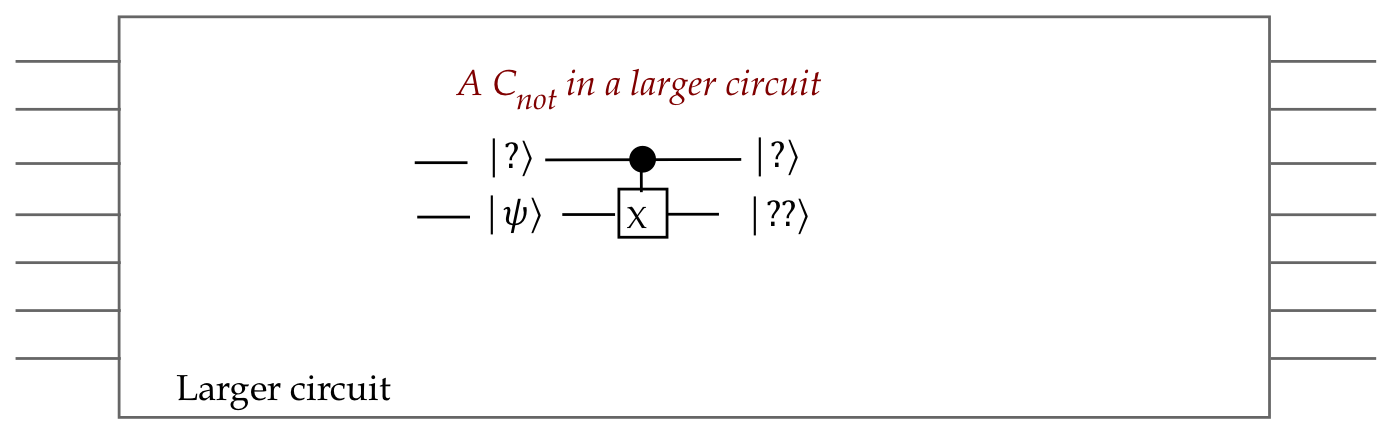
\includegraphics[width=4in]{notes/figs/n08/48caveat2.png}
        \caption{$C_{NOT}$ embedded gates}
        \label{fig:48caveat2}
    \end{figure}
    
    This raises the question: what is the guarantee that the inputs to such a $C_{N O T}$ are what it expects? In a later module we will see this question resolved as follows: Circuits will be designed with S-basis reasoning. Yet superpositions will be supplied as input. We'll then use linearity to determine the output. For example, suppose a circuit $U$ has been designed with four qubits and its effect is known on the standard basis $|0000\rangle, \ldots,|1111\rangle$. Now suppose we supply as input the superposition
    
    $$
    |\psi\rangle=\frac{1}{\sqrt{2}}(|0000\rangle+|1111\rangle)
    $$
    
    Then,
    
    $$
    U|\psi\rangle=U \frac{1}{\sqrt{2}}(|0000\rangle+|1111\rangle)=\frac{1}{\sqrt{2}}(U|0000\rangle+U|1111\rangle)
    $$
    
    We can now reason about the output because we know $U|0000\rangle$ and $U|1111\rangle$ on these standard-basis vectors. One needs to be careful in reasoning about global versus local phase in the multi-qubit context: Consider the difference between $|1\rangle \otimes|0\rangle$ and $|1\rangle \otimes K(\delta)|0\rangle$ : We may reason that
    
    $$
    K(\delta)|0\rangle=e^{i \delta}|0\rangle=|0\rangle
    $$
    
    because of global-phase. Then $|1\rangle \otimes K(\delta)|0\rangle=|1\rangle \otimes|0\rangle=|10\rangle$ with this reasoning. Now let's apply tensoring properties
    $|1\rangle \otimes K(\delta)|0\rangle=K(\delta)(|1\rangle \otimes|0\rangle)=e^{i \delta}(|1\rangle \otimes|0\rangle)=e^{i \delta}|10\rangle=|10\rangle$. So it appears to work in this case. However, if instead this was part of a superposition:
    
    $$
    \frac{1}{\sqrt{2}}(I|01\rangle+|1\rangle \otimes K(\delta)|0\rangle)=\frac{1}{\sqrt{2}}\left(|01\rangle+e^{i \delta}|10\rangle\right) \neq \frac{1}{\sqrt{2}}(|01\rangle+|10\rangle)
    $$
    
    In this case, the factor $e^{i \delta}$ cannot be ignored. One cannot treat quantum circuits like classical circuits even with standard-basis qubits: Consider this example in Figure \ref{fig:49caveat3}.
    
    \begin{figure}
        \centering
        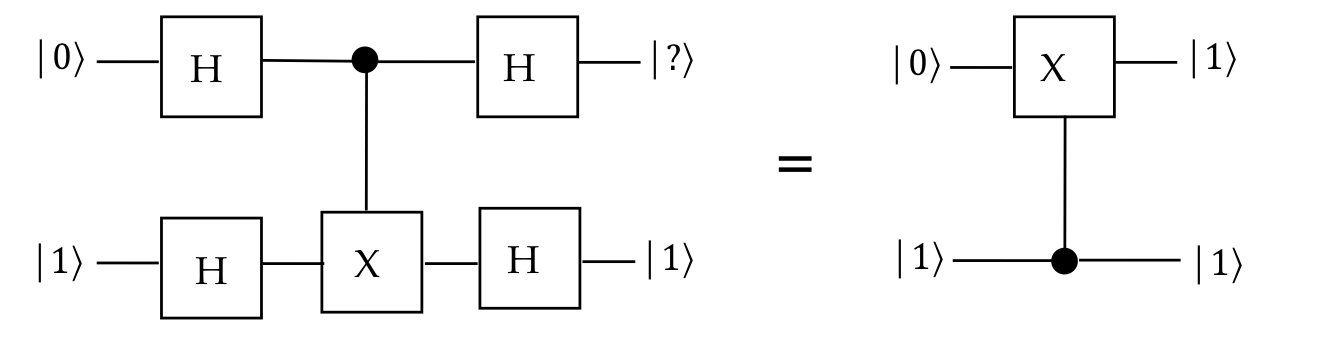
\includegraphics[width=4in]{notes/figs/n08/49caveat3.png}
        \caption{Quantum Classical Differences}
        \label{fig:49caveat3}
    \end{figure}

\end{document}